\documentclass[a4paper,12pt]{report}

\usepackage{lmodern} %Latin Modern
\usepackage{xspace} 
\usepackage{etoolbox}
\usepackage[T1]{fontenc}
\usepackage[page,toc]{appendix}
\usepackage{graphicx}
\usepackage{subcaption} %provide caption for each sub figure
\usepackage[hyphens]{url}
\usepackage{paralist} %inline list
\usepackage{hyperref} %clickable links
%Options: Sonny, Lenny, Glenn, Conny, Rejne, Bjarne, Bjornstrup
\usepackage[Bjornstrup]{fncychap}
\usepackage{tabu}
\usepackage{booktabs}
\usepackage{tikz}
%ams
\usepackage{amsthm}
\usepackage{amsmath}
\usepackage{amsfonts}
\usepackage[autolanguage]{numprint} % print formatted number
%lcode isting
\usepackage{listings}

\definecolor{mygreen}{rgb}{0,0.6,0}
\definecolor{mygray}{rgb}{0.5,0.5,0.5}
\definecolor{mymauve}{rgb}{0.58,0,0.82}

\lstset{ %
	backgroundcolor=\color{white},   % choose the background color
	basicstyle=\footnotesize,        % size of fonts used for the code
	breaklines=true,                 % automatic line breaking only at whitespace
	captionpos=b,                    % sets the caption-position to bottom
	commentstyle=\color{mygreen},    % comment style
	escapeinside={\%*}{*)},          % if you want to add LaTeX within your code
	keywordstyle=\color{blue},       % keyword style
	stringstyle=\color{mymauve},     % string literal style
}

\usepackage[font={footnotesize}]{caption}
\usepackage{color}
%fancy framed box
\usepackage{tcolorbox}
\usepackage{pdfpages}
\usepackage{biblatex}
\bibliography{ref.bib}

\usepackage{glossaries}

\newcommand*\justify{%
	\fontdimen2\font=0.4em% interword space
	\fontdimen3\font=0.2em% interword stretch
	\fontdimen4\font=0.1em% interword shrink
	\fontdimen7\font=0.1em% extra space
	\hyphenchar\font=`\-% allowing hyphenation
}

% numbers subsubsection
\setcounter{secnumdepth}{3}
\setcounter{tocdepth}{1}

\title{Procedural Generation of Tactical RPG Battle Systems}
\author{Worakarn Isaratham\\140024714}

%macro to let later reference to values of \title and \author
\makeatletter
\let\inserttitle\@title
\let\insertauthor\@author
\newcommand*{\rom}[1]{\expandafter\@slowromancap\romannumeral #1@}
\makeatother

\makeglossaries
\renewcommand*\glspostdescription{\dotfill}
\renewcommand{\glossarysection}[2][]{}
 
\newglossaryentry{gta5}
{
    name={Grand Theft Auto \rom{5}},
    description={Rockstar Games. 2013}
}

\newglossaryentry{starwars-tor}
{
	name={Star Wars: The Old Republic},
	description={Electronic Arts. 2011}
}

\newglossaryentry{destiny}
{
	name={Destiny},
	description={Activision. 2014}
}

\newglossaryentry{rogue}
{
	name={Rogue},
	description={Michael Toy, Glenn Wichman, Ken Arnold. 1980}
}

\newglossaryentry{angband}
{
	name={Angband},
	description={Alex Cutler, Andy Astrand. 1990}
}

\newglossaryentry{diablo}
{
	name={Diablo},
	description={Blizzard Entertainment. 1996}
}

\newglossaryentry{dwarffortress}
{
	name={Dwarf Fortress},
	description={Bay 12 Games. 2006}
}

\newglossaryentry{spelunky}
{
	name={Spelunky},
	description={Mossmouth. 2008}
}

\newglossaryentry{civ}
{
	name={Civilization},
	description={MicroProse. 1991}
}

\newglossaryentry{fireemblem}
{
	name={Fire Emblem},
	description={Nintendo. 1990}
}

\newglossaryentry{fft}
{
	name={Final Fantasy Tactics},
	description={Square. 1997}
}

\newglossaryentry{disgaea1}
{
	name={Disgaea: Hour of Darkness},
	text={Disgaea},
	description={Nippon Ichi Software. 2003}
}

\newglossaryentry{warcraft}
{
	name={Warcraft: Orcs \& Humans},
	text={Warcraft},
	description={Blizzard Entertainment. 1994}
}

\newglossaryentry{cnc}
{
	name={Command \& Conquer},
	description={Virgin Interactive. 1995}
}

\newglossaryentry{starcraft}
{
	name={Starcraft},
	description={Blizzard Entertainment. 1998}
}

\newglossaryentry{zog}
{
	name={Zillions of Games},
	description={Zillions Development Corp. 1998}
}

\newglossaryentry{yavalath}
{
	name={Yavalath},
	description={Cameron Browne. 2007}
}

\newglossaryentry{runescape}
{
	name={RuneScape},
	description={Jagex. 2001}
}

\begin{document}

%TC:ignore 

\begin{titlepage}

\begin{center}
	
	\Huge
	{\bfseries \inserttitle}\\[1.5cm]
	
	\Large
	\insertauthor\\
	
\includegraphics[width=0.5\textwidth]{standrews_logo}\\
	\small
	This dissertation is submitted in partial fulfilment\\
	for the degree of\\
	\normalsize
	Erasmus Mundus MSc Dependable Software Systems\\
	\small
	at the\\
	\normalsize
	University of St~Andrews\\
	\small
	under supervision of\\
	\normalsize
	Prof. Ian Miguel\\[1cm]
	\today\\[0.5cm]
	
\includegraphics[width=0.3\textwidth]{erasmus_mundus_EU}\\[2cm]
	
\end{center}

\end{titlepage}

%%% PATCHES %%%
% http://tex.stackexchange.com/questions/109708/initial-page-numbers-wrong
\makeatletter
% Patch `titlepage` not to reset the page number
\patchcmd{\titlepage}{\setcounter{page}\@ne}{}{}{}
\patchcmd{\endtitlepage}{\setcounter{page}\@ne}{}{}{}

% Patch `abstract` so that it shows the page number
\patchcmd{\abstract}{\titlepage}{\titlepage\thispagestyle{plain}}{}{}
\makeatother
%%% END PATCHES %%%

\newcommand{\gameref}[1]{\emph{\gls{#1}}}

\pagestyle{plain}
\pagenumbering{roman}

\renewcommand{\titlepage}{\relax}

\renewcommand{\abstractname}{Declaration}
\begin{abstract}
	
	I, Worakarn Isaratham, hereby certify that this dissertation, which is approximately \input|"./count.sh" words in length, has been written by me, and that it is the record of work carried out by me, or principally by myself in collaboration with others as acknowledged, and that it has not been submitted in any previous application for a higher degree. The higher study for which this is a record was carried out in the University of St Andrews during the current academic year.\\[2cm]
	
	\begin{flushright}
		\rule{0.3\textwidth}{0.4pt}
		
		Worakarn Isaratham\\
		\today
	\end{flushright}
\end{abstract}

\renewcommand{\abstractname}{Acknowledgements}
\begin{abstract}
	
TBD
	
\end{abstract}

\renewcommand{\abstractname}{Abstract}
\begin{abstract}
	
Making games is expensive, and much of the resources is spent on creating game content. Procedural generation is a method that enables game content to be generated algorithmically and automatically, rather than manually. Common application of this technique is currently being used for low-level content such as textures, vegetation, clouds, game maps, road networks, or puzzles. This work attempted to apply procedural generation to a higher-level content, in the context of tactical role-playing games (TRPG). Central to games in this genre are turn-based battles between game characters, which resemble complex chess-like board games. The complexity of the battles arises from the variety of game characters, and the combat actions they can perform. Crucial to the enjoyment of the game is the balance between all the available choices of characters and actions, which we collectively call the battle system. Calibrating the system to be in balance is usually done manually. Instead, we created a prototype TRPG battle, and a procedure that algorithmically generates a well-balanced battle system for the prototype. An objective function was defined, based on self-play game AI, to evaluate all possible battle systems as numerical values. We then used genetic algorithm to optimise the objective function, to find the battle system that fits the objective best. Finally, we had human volunteers play the game running on various battle systems, to validate that the procedurally-optimised one is in good balance.
	
\end{abstract}

\tableofcontents

\newpage

\pagenumbering{arabic}

\justify

%TC:endignore 

\chapter{Introduction}

\section{Background and motivation}

\subsection{Procedural generation in games}

The industry of computer games is a big and serious business, even bigger than those of film and music.\cite{web-gamebigindustry} The global market size was estimated to be 83 billion USD in 2014, and is expected to surpass 100 billion by 2018.\cite{web-gamesmarket2018} Not only the revenue is growing, producing a game is also becoming increasingly expensive. \gameref{gta5} (2013), for example, has the production cost of 265 million USD, including both development and marketing.\cite{web-gta5}

Much of the development cost of a video game can be attributed to \textit{content generation}, estimated from anecdotal evidences to be in the range of 30\%--40\% of total budget.\cite{hendrikx2013procedural} The generated content covers everything from elementary bits and pieces -- textures, sound, vegetation, etc. -- to more sophisticated ones such as maps, stories, puzzle elements, and even the rules of the game themselves. It usually takes large teams of highly-skilled human creators to produce game content. \gameref{starwars-tor} (2011), whose development cost alone was estimated to be almost 200 million USD, was developed by teams of more than 800 people across four continents, for 6 years.\cite{web-oldrepublic} For \gameref{destiny} (2014) it took around 500 people to manually create most of the content.\cite{web-expensivedevelop}

With the amount of resources -- both time and money -- currently being spent to create content for modern games, it is tempting to try to do it automatically, rather than manually. \textbf{Procedural generation} is a technique that aims to accomplish this. Togelius et al.\cite{togelius2011procedural}\ defined procedural generation as `the creation of game content automatically using algorithms'\footnote{The actual definition is for the term \textbf{procedural content generation}, as opposed to \textbf{procedural generation}, which in some context is limited to only the process of generating content that does not affect gameplay \textit{significantly}. (See \url{http://pcg.wikidot.com/pcg-algorithm:procedural-generation}) However, in this work these two terms will be used interchangeably.}. Historically, the motivation for procedural generation was not always about cost reduction. Computer programs used to operate at extremely limited amount of memory. Procedural generation helps in this aspect by producing large amount of content dynamically at run-time, effectively packing a lot of information into very small amount of memory, comparing to static content. Moreover, since procedural-generated content is generated randomly, it increases variety, and thus replayability for the games. %citation?

Various types of game content have been created procedurally since the early days of video games. The roguelike genre and its relatives -- games such as \gameref{rogue} (1980), \gameref{angband} (1990), \gameref{diablo} (1996), or \gameref{dwarffortress} (2006) -- all feature adventures in procedural-generated dungeons. \gameref{spelunky} (2008) also uses procedural generation to create its dungeon, but in a vertical 2-D, platformer style. Maps in the strategy game series \gameref{civ} (1991) are also generated procedurally, and play a crucial role in the massive success of these games\cite{web-7usesofprocgen}. Another example of success application of procedural generation is \textit{SpeedTree}, a tool that generates vegetation procedurally. It has been used extensively in commercial games, and also in film industry -- starting from James Cameron's \textit{Avatar} in 2009.\cite{web-speedtree}

\begin{figure}
	\centering
	\includegraphics[width=.7\linewidth]{figures/Spelunky.png}
	\caption{A procedurally-generated vertical level in \textit{Spelunky}.}
\end{figure}

\subsection{Tactical role-playing game}

Tactical role-playing game (TRPG) is a sub-genre of role-playing game (RPG)\cite{stenstrom2013understanding}, but also sometimes classified as a type of strategy wargame, incorporating elements from both genres. It is also known as \textit{strategy RPG}, or \textit{simulation RPG}.\cite{web-srpg} Classic examples of the genre include \gameref{fireemblem} (1990), \gameref{fft} (1997), and the \gameref{disgaea1} franchise (2003)\cite{web-playingroles}.

\begin{figure}
	\centering
	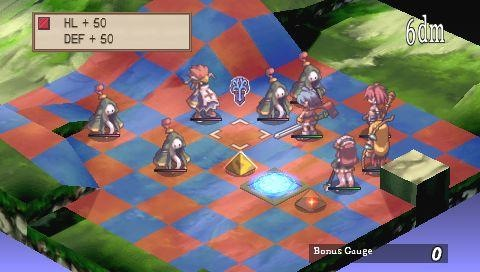
\includegraphics[width=.7\linewidth]{figures/disgaea_aod.jpg}
	\caption{A battle scene from the tactical RPG \textit{Disgaea: Afternoon of Darkness}.}
\end{figure}

Among the various sub-genres of RPG, tactical RPG could be characterised as the one with the strongest emphasis on combats, at the expense of world exploration.\cite{stenstrom2013understanding} The focus of a TRPG is on battle scenes, which take place on some sort of grids (usually square), where two players each take control of a party of units, moving them around and attacking or defending from the other party. The same description could also be used to describe strategy games, spanning from abstract strategy board games such as chess, checkers, or go, to the modern computer games in the genre of \textit{real-time strategy} (RTS), such as \gameref{warcraft} (1994), \gameref{cnc} (1995), or \gameref{starcraft} (1998). TRPG has so much in common with the strategy games, that it is sometimes called `mini-wargame', and grouped together with strategy games rather than RPG.\cite[92, 108]{moore2011basics} The key difference that distinguishes RPG from strategy, however, is that of \textit{perspectives}. In RPG, players are asked to identify with a character (or a party of characters), while in strategy games, characters are treated more like dispensable resources that are produced from some sort of factories.\cites[8]{barton2008dungeons}[455]{adams2010fundamentals} In this sense, TRPG definitely belongs to the RPG genre.

The complexity of a TRPG arises from the range and combination of moves and actions each unit can perform. In contrast to other types of RPG where battles are trending towards being real-time, TRPG retains the primary turn-based nature of traditional tabletop RPG.\cite[90]{moore2011basics} This allows players to plan and experiment with different options, favouring tactical skills over responsiveness.

\subsection{Game balance}

Balance is one of the most crucial part of any games. It is considered to be the most subtle part of game design; an art, rather than science.\cite{schell2008art} As TRPG focuses so heavily on the combats, one of the primary aspects that need to be in balance is the effect of each of the choices available to the players on the combat, which we collectively call the \textbf{battle system}. This includes things such as classes and races of the characters, strength and attacking range of weapons, effectiveness of armours against different types of attacks, etc.

Striking good balance is usually carried out by a long and tedious process of \textit{manual testing} and \textit{fine-tuning}. Automating the process would potentially lead to rewarding benefits. %some ref here would be nice
However, procedural generation tends to be used more on peripheral aspects of games; producing texture, sounds, vegetation, and maps, are some of the most common applications.\cite{hendrikx2013procedural} Battle systems, on the other hand, are central to the gameplay of TRPG, and has not been explored as much. This leads us to ask:

\begin{tcolorbox}
	How can procedural generation be used to create balanced battle systems for tactical role-playing games automatically?
\end{tcolorbox}

This is the main research question that this work will attempt to address.

\section{Objectives}

The aim of this work is to study the possibility of using procedural generation to generate battle systems in a balanced way. To achieve this, the following objectives are the primary ones that need to be met:

\begin{itemize}
	\item A \textbf{prototype TRPG}, as a playable game on its own. As our focus is solely on the battles, other aspects of typical TRPG such as character progression or storytelling can be ignored. To allow human players to play the game and observe the ensuing battles, a user interface for the game is required, though it does not have to be sophisticated -- a simple command line interface, for example, would suffice.
	
	\item The \textbf{battle mechanics} of the prototype must support these minimal aspects of typical TRPG gameplay:
	\begin{itemize}
		\item Battles are won by removing all the opponent's units.
		\item Characters possess a small set of basic attributes that builds up more complex ones.
		\item Standard action types are supported: physical melee attack, long range attack, magical attack, and healing.
	\end{itemize}

	\item An \textbf{AI player}. It is an essential part of the battle system evaluation process. The AI must be generic enough to play the game for any generated battle systems, in a reasonably competent manner.
	
	\item A \textbf{procedural generation program} that creates balanced battle systems for this TRPG. Ideally, game designers -- the target users of this program -- would express the game balance as a set of conditions. The program would take these as inputs, and try to create a battle system that satisfies the balance conditions.
	
\end{itemize} 

Secondary objectives that are not required, but would be valuable additions to the project, are:
\begin{itemize}
	\item A graphical user interface.
	\item Races and jobs systems.
	\item More complex battle mechanics, such as magical spells that cause or cure status abnormalities, or incorporation of terrain height and/or type into calculation (e.g. melee attack cannot reach higher tiles, lava tiles drain hit points from units). 
\end{itemize}

\section{Outline}

The rest of this dissertation will be organised as follows. First, previous work in this area that is relevant to our goals will be explored in chapter 2. Chapter 3 will lay out the design of the solution to our research question. The implementation of that design will be described in chapter 4. The solution will then be evaluated in chapter 5. Finallly, the last chapter will conclude the result, and suggest future developments that could build upon this work.
\chapter{Related Work}

In the first chapter we have touched upon the history of usage of procedural generation in game creation. A comprehensive exploration of the current stage of procedural generation in games can be found in \cite{pcgbook}. In this chapter we will be more focused, exploring more closely on existing use of this technique in circumstances similar to that of our research question.

\section{Procedurally-generated game design}

First we try to contextualise TRPG battle systems within the landscape of game content generation. Hendrikx et al.\cite{hendrikx2013procedural}\ identified six levels of content, as shown in figure \ref{fig:pyramid}. Content at the bottom of the pyramid is more elementary and peripheral, whereas the upper classes are more complex entities. Under this scheme, TRPG battle systems can be classified under \textit{system design}, a part of the \textit{game design} layer within the pyramid. System design is defined as `the creation of rules and underlying mathematical patterns in a game'\cite[5]{brathwaite2009challenges}, which is definitely a fit description of TRPG battle systems.

\begin{figure}
	\centering
	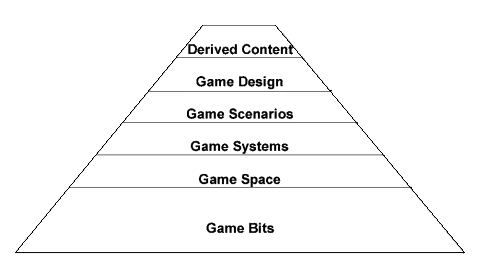
\includegraphics[width=.6\linewidth]{figures/PCG_pyramid}
	\caption{Layers of procedurally-generated game content. (adapted from \cite{hendrikx2013procedural})}
	\label{fig:pyramid}
\end{figure}

Some work does not focus on generating the game rules themselves, but rather how to combine and match the rules to concrete representations. A notable example is  \textbf{EGGG}\cite{orwant2000eggg}. This automatic programming system takes a minimal descriptive rule set of a game, written in a domain specific language, then `fleshes out' the game by using heuristics to fill in details of the rules, and packaging it as a playable game, complete with graphical user interface and an AI opponent.

Closer to our interest are works that focus on generating the whole set of rules for the games. An early example, \textbf{METAGAMER}\cite{pell1992metagame}, is a system that generates games in the class of `symmetric chess-like board games', developed  with the purpose to encourage game AI development away from being too specific to a game (such as chess) and into the direction of general game-playing. METAGAMER uses a game grammar that describes a wide range of games, and for its purposes of creating more games for the AI to play, there was no need to give preferences to any specific properties -- game instances were merely picked at random.
	
Hom and Marks\cite{hom2007automatic} extended the idea, by describing a system that also generates board games, but with a specific goal of \textit{balance}. Board games are described using Lisp-like description language originally created for \gameref{zog} -- a commercial general board game playing system, developed by Jeff Mallett and Mark Loeffler.\cite{levy2005robots} Genetic programming is then used to evolve a population of games using a fitness function that measure games balance.

The idea of using evolutionary algorithm (of which genetic algorithm / genetic programming are subtypes) to measure the quality of generated games has since become common. Ludi\cite{browne2010evolutionary} is a complete system that generates, evaluates, and creates playable user interface, using evolutionary approach. Games are described using its own general game playing description language. Rules are evolved using genetic programming, as shown in figure \ref{fig:ludi}. Standard genetic operations of crossover and mutation are applied to the population of games, then surviving games are evaluated, using a large number of criteria. The success of Ludi is proven by the fact that \gameref{yavalath}, one of the games generated from the system, has been published commercially, and was ranked in the top 100 abstract strategy board games ever invented.\cite{browne2011yavalath}

\begin{figure}
	\centering
	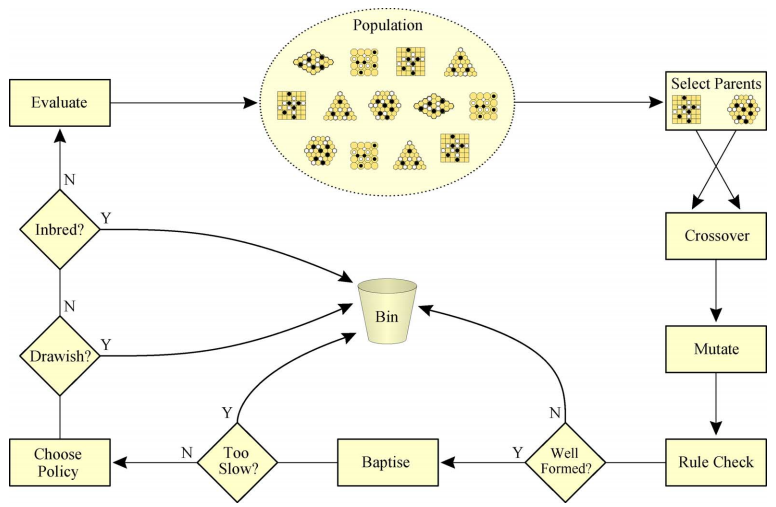
\includegraphics[width=.8\linewidth]{figures/ludi}
	\caption{Evolution process for games in Ludi system. Figure taken from \cite{browne2010evolutionary}.}
	\label{fig:ludi}
\end{figure}

\begin{figure}
	\centering
	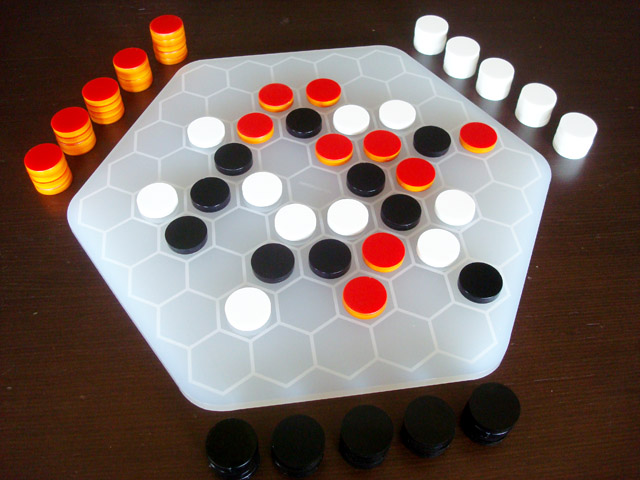
\includegraphics[width=.8\linewidth]{figures/yavalath.jpg}
	\caption{\textit{Yavalath}, a commercial game generated from Ludi.}
	\label{fig:yavalath}
\end{figure}

Progress has also been made on generating game rules for graphical video games. An experimental system by Togelius and Schmidhuber\cite{togelius2008experiment} was able to generate discrete, Pacman-like games, also by using evolutionary algorithm. Variations Forever\cite{smith2010variations} instead uses \textit{answer set programming}, a form of logic programming, to generate rule sets of graphical 2-D video games that satisfy given constraints, without using evaluation function. In the same manner that game description languages, originally created for general game-playing AI development, have been used to evolve abstract board games, Video Game Description Language (VGDL)\cite{ebner2013towards}, which was proposed to assist in \textit{general video game playing}, could also be exploited to generate video games.

Similar efforts to extend or create game description languages have been done on several other domains, and therefore can also be used for game generation. These includes card games\cite{font7835card}, action-adventure games\cite{dormans2012generating}, puzzles\cite{web-puzzlescript}, general real-time games\cite{kowalski15game}, and strategy games\cite{mahlmann2011towards}.
	
\section{Procedural generation in strategy games}

To the best of our knowledge, procedural generation has never been attempted in the specific case of TRPG battle systems. However, works in related genres exist. In one sense, TRPG battles can be thought of as more complex board games, which have been a primary subject of procedural generation research, as already presented in the previous section. In another perspective, TRPG battles are very similar to turn-based strategy games. There exists research in using procedural generation on strategy games, though not as extensive as in board games.

Some of these works\cites{togelius2010multiobjective, liapis2013generating} focus on the task of \textit{map generation} in games such as \gameref{starcraft}. Maps play a big role in strategy games in general, since the positions of resources required for various activities do influence how the game might progress. In contrast, such resources usually do not exist in TRPG, and while TRPG battle maps do affect the positioning of units, which in turn could affect the effectiveness of units' skills, they are not as influential.

Another work by Mahlmann et al.\cite{mahlmann2011towards}\ explores the balance of units in turn-based strategy games. First they developed the Strategy Game Description Language (SGDL) to describe a landscape of strategy games, then developed an AI that is able to play any games defined in SGDL, and use genetic programming to create a balanced set of units for a simplistic strategy game. The fitness function used in the evolution was based on the damage each type of unit can inflict upon each other. Based on this successful result, if SGDL is extended further to include other aspects of strategy games, then it could be possible to automatically generate all aspects of this type of games.

\section{Discussion}

In this chapter we have looked into the attempts to use procedural generation techniques to create game content at a level similar to that of TRPG battle systems. Search-based procedural generation techniques -- in particular evolutionary programming with simulation-based fitness function -- are common, since evaluation of the generated content at the level of game rules and mechanics is difficult (or impossible) to achieve without actually experiencing the games in some way.\cite{togelius2010search} A number of these systems operate at a level above any specific game, using a game description language to describe a large set of games. Game rules have been generated for different domains, such as abstract board games, graphical 2-D video games, and, most interesting for our purposes, strategy games.

For the scope of this work, we will focus on a single prototypical game as a representation of TRPG battles, therefore a game description language is not needed. Evolutionary algorithm, however, appears to be a successful paradigm for this kind of task, and therefore would be adopted as our main approach to the solution of our research question, the design of which will be explored in the next chapter.
\chapter{Solution design}

The primary objectives stated in the first chapter mention a few artefacts that are components of the solution to the research question, such as the TRPG prototype, the AI player, and the battle system generator. In this chapter we present the design of the solution -- how these artefacts will be built and connected together, and how will they be used to create balanced battle systems.

\section{High-level design}

\begin{figure}
	\centering
	\includegraphics[width=.8\linewidth]{figures/TRPG_flow.png}
	\caption{Relationship between subsystems of the prototype.}.
	\label{fig:flow}
\end{figure}

The solution will be composed of the following subsystems, with relationship as shown in the diagram in figure \ref{fig:flow}.
\begin{itemize}
	\item \textbf{The TRPG prototype battle model.} A player would need to go through a lot of battles in a normal TRPG. However, since all aspects of the genre other than the battles are ignored for the scope of this project, it is adequate for the game prototype to model only a single battle. The model will include all components of the battle -- the combat rules, game board, players, weapons, armours, units, and the unit attributes. The rules will be rather fixed, as opposed to a more generalised approach seen in the previous chapter, to minimise the complexity of the battle system.
	\item \textbf{The battle system} describes the parameterised parts of the model. Its purpose is to make the model adjustable, in order to accomplish a certain goal. These parameters control numerical calculations, such as how the unit basic attributes are combined into more complex ones, or how the quality of weapons and armours are factored into damage calculation.
	\item \textbf{The battle controller} connects the players to the game model. It controls the progress of the battle, by determining the next unit to move, asking for battle commands from the associated player, and adjusting the state of the battle accordingly.
	\item \textbf{The user interface} redirects battle commands from the human player to the controller, and displays the progress of the battle.
	\item \textbf{Constrained battle generator} produces random battles under a given set of constraints, such as the types of units available to each player, or the distribution of basic attributes for the units.
	\item \textbf{The AI player} selects battle commands automatically, by trying to evaluate each possible options and choose the one that maximises its chance to win the battle.
	\item \textbf{Battle system objectives and evaluator}. The objectives establish the criteria for evaluation. The main objective is to make the system in balance, and since the concept of \textit{balance} might be interpreted in several ways, this goal is likely to contain multiple subgoals. Evaluation is to be done by simulating several battles under the constraints specified by the objectives, letting the AI player plays against itself, and assessing the outcome of the battle against the objectives.
	\item \textbf{Battle system optimisation procedure} -- the procedure that tries to systematically produce an optimal battle system. While the primary choice is genetic algorithm, other search-based, simulation-based procedure can also be used.
\end{itemize}

\section{The battle model}

The battle model is the complete description of the battle happening in the TRPG prototype. It defines all the rules and components of the game. The prototype attempts to incorporate into the battle model many of the common components found in typical TRPGs, but the variation will be kept small and simple..

\subsection{The battlefield}

Battles take place on a \textit{battlefield}, which is a rectangular grid. A fraction of the cells are filled with obstacles, thus inaccessible to the playable units. For each of the accessible ones, there is an associated \textit{height}. Two accessible cells are \textit{connected} if they are orthogonally adjacent, and the difference in height is not too much (no larger than 1). This affects the range of movement of the playable units, as will be described in section \ref*{sub:playsequence}.

The heights and the inaccessible portions are randomly generated, but in such a way that it is guaranteed that the battlefield is fully connected -- that is, there always exists a path for a unit to move from one accessible cell to another.

\subsection{The battle objective}

A typical TRPG battle is played out between two parties of units. In actual commercial games there are different kinds of battle objectives, such as `unit $x$ must not die', `kill unit $y$', or `survive the battle for $n$ turns'. In this prototype every battle has the same objective: `eliminate the other party'. To be precise, a unit is removed from the battle when its \textit{hit points} (HP) reaches zero, and when a party has all its units removed then that party loses the battle.

\subsection{Playable units}

A unit is a playable character that players can control, move them around the battlefield and make them perform battle actions. Units are differentiated mainly by their \textit{attributes} and the type of actions they can perform.

\subsubsection*{Character attributes}

Character attributes, also known as \textit{stats}, are the usual basis of combat resolution.\cite[94]{moore2011basics} In this prototype the fundamental ingredients of all the character attributes are the five \textit{basic attributes}, adopted from the game \gameref{angband}. They are: strength, intelligence, wisdom, dexterity, and constitution.\cite{sw-angband} All other attributes are functions of either one or two of the basic attributes. For example, \textit{speed} is a function of dexterity alone, while \textit{physical attack} is a function of strength and constitution. The exact form of these functions is details which form a major part of the battle system.

\subsubsection*{Races}

In addition to intrinsic values given to the basic attributes when generating the units, the choice of \textit{race} modifies the values further. The concept of races is common in RPG, with mythological races for fantasy settings, or extraterrestrial races for a sci-fi theme. Each race possesses different natural traits and abilities. For examples, \textit{elves} are usually portrayed as small, elusive creatures that are physically weak, but very proficient in magic. There are many kinds of racial effects, but in this prototype they are restricted to the following:
\begin{enumerate}
	\item Modification to basic attributes -- bonuses and penalties given to each race, in a balanced way. For example, humans have no modification at all, while elves have one point added to their dexterity and intelligence attributes, and one point deducted from their strength and constitution. In both cases, as well as in all other races, the sum of points modified is zero.
	\item Character's weight. This attribute sets a soft limit of the total equipment weight worn by the unit. Going over this limit will slow the unit down, affecting its place in the sequence of play, as will be explained in section \ref{sub:playsequence}.
\end{enumerate}

\subsubsection*{Jobs and equipment}

Similar to races, jobs (or \textit{character classes}) also provides differentiation to the units. In modern RPG, characters can usually change jobs to gain a wide range of abilities, whereas races are fixed throughout the game. In this prototype jobs have a single function: limiting the type of \textit{equipment} units can wear. 

Equipment is all the items that the characters can wear or wield, categorised by body parts. Typically this means a swordman character might equip, for example, a sword in one hand, a shield in the other hand, a chainmail, a pair of gloves, a pair of shoes, a helmet, and a magical ring. Since there is no in-battle equipment change mechanism, this simple prototype downplayed the role of equipment. As a result, a unit can wear only two pieces of equipment --  one weapon and one body armour/clothing. 

Armours provide additional protection to the units, while weapons provide the offensive power. Another important function of the weapons is to dictate the type and range of attack a unit can do, which means that a unit's attacking ability is an indirect consequence of its job.

The following is the list of all four jobs in this prototype, with their associated equipment:
\begin{itemize}
	\item \textbf{Warriors} are specialised in close-ranged combat. They use \textit{melee} weapons such as swords or lances, wear \textit{plate armours}, and have no magical abilities.
	\item \textbf{Rangers} are \textit{long-range} combat specialists. They fire projectiles from afar, wear clothes made from \textit{hide}, and also have no magical abilities.
	\item \textbf{Mages} are users of black magic. They can cast magic spell to attack opponents, and their magical staves can also be used as blunt weapons. Unlike the warriors and rangers they do not use protective gears, instead they wear simple mages' \textit{robes}.  
	\item \textbf{Clerics} are also magic users with similar kind of equipment to the mages. The difference is that their white magic can only be used to heal, not to harm. Their staves can still be used as physical weapons though.
\end{itemize}

All types of weapons are capable of making physical damage. The attacking range of each weapon type is detailed in table \ref{table:attacking_range}. Most weapons have close-ranged physical attack, effective only on the cells immediately adjacent to the unit. The exception is the bows, which are effective on cells further away and \textit{not} on the immediately adjacent cells.

\begin{table}
	\begin{tabu}{X[l2] X[l3] X[l8] }
		\toprule
		weapon & wielded by & cells in attacking range, if the attacker is at $(x, y)$\\ 
		\midrule
		unarmed & all & $(x, y \pm 1), (x \pm 1, y)$\\
		sword & warriors & $(x, y \pm 1), (x \pm 1, y)$\\
		lance & warriors & $(x, y \pm 2), (x, y \pm 1), (x \pm 2, y), (x \pm 1, y)$\\
		bow & rangers & $(x', y')$ such that $2 \leq |x'-x| + |y' - y| \leq 5$\\
		staff & mages, clerics & $(x, y \pm 1), (x \pm 1, y)$\\		
		\bottomrule
	\end{tabu}
	\caption{Attacking range for each type of weapon}
	\label{table:attacking_range}
\end{table}

Target range for magical spell works in a similar way to long-range attack, with the range of spells fixed at 0--6 squares. The minimum range of 0 enables the spellcaster to be the target of its own spell, allowing clerics to do self-healing.

Balancing the jobs is the main focus of this work. It will be explored in details in section \ref{sub:battleobjectives}.

\subsubsection*{Magic system}

Magic is very common in games with fantasy settings. There are many different kinds of magic, but in this prototype the two most-common ones are used: black magic and white magic. Black is attacking magic, which can only be used by mages. White is healing magic employed by clerics. Black magic is further sub-divided into subtypes based on three different magical elements: \textit{fire}, \textit{water}, and \textit{nature}. Fire has inherent advantage over nature, which beats water, which in turn beats fire. Some armours are magically-enhanced, making them more resistant toward an element, but also weaker against another. 

Each spell has 3 levels, with the higher-level ones being stronger and costing more \textit{magic points} (MP). The exact relationship between the spell-level and the effects is left to be defined by the battle system.

\subsection{Sequence of play}
\label{sub:playsequence}

TRPG in general employs turn-based combat system. The order of turns are resolved in a few different flavours. A simple system takes turns between the two players, with each player allowed to move all the units in command at once. More complex systems are finer-grained, regulating turns on unit-level rather than party-level.

One such fine-grained system used in \gameref{fft}\cite{web-fftbmg} was adopted for this prototype. The sequence of turns depends solely on the \textit{speed} attribute of the units. In this system, a unit gets its turn once its \textit{charge time} gauge is full (breaking ties arbitrarily), and the gauge is emptied after the unit has finished its turn. Speed indicates how fast the gauge gets filled in one time unit. This system allows a unit to receive multiple turns before another unit can act, making the speed attribute a highly-influential one.

Once its turn has arrived, every unit has an opportunity to do two actions:
\begin{enumerate}
	\item Move to another cell within a legal range.
	\item Carry out an operation, which could be a physical attack or a spell casting. 
\end{enumerate}
Neither options are required, so the unit can perform both, or choose one, or just skip the turn. The order of actions are also not restricted -- it is both possible to move into a new position then attack, or to attack first then move away.

\begin{figure}
	\centering
	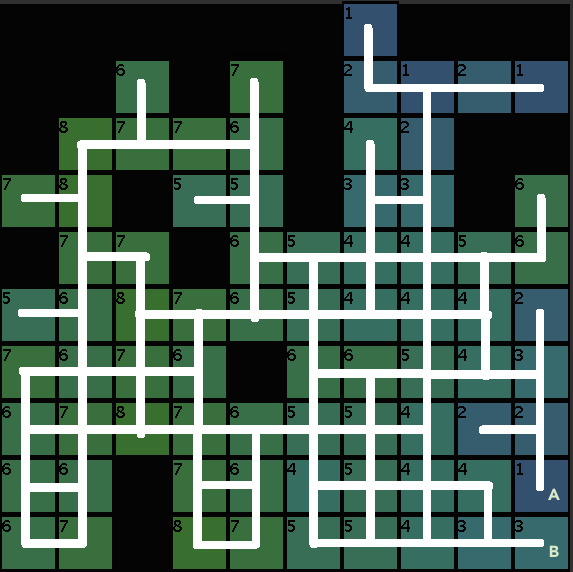
\includegraphics[width=.6\linewidth]{figures/connections}
	\caption{A battlefield, considered as a connected graph. The distance between points A and B at the bottom-right, despite the two points looking seemingly adjacent, is actually 9.}
	\label{fig:connected}
\end{figure}


The legal cells that a unit can move to are determined by the attribute \textit{move range}, which is a small positive integer. If we consider the battlefield as a connected graph with cells as vertices (figure \ref{fig:connected}), then given the move range $n$ the legal cells are all vertices whose shortest path from the current cell is at most $n$ cells away.

\subsection{Excluded elements}

There are some common characteristics of TRPG that are left out of this prototype.

\begin{itemize}

\item Experience system. Characters in RPG usually gain higher attributes or new skills from \textit{experience}. An experience system works by giving characters experience points from accomplishments, such as winning battles or completing quests. The points can then be converted into new abilities or increasing attribute values.

\item Equipment change within the battle, as another type of action in addition to attack and magic.

\item Items usage can also be added as another type of action.

\end{itemize}

 These are all common RPG traits. Including them, however, would elevate the level of complexity of the prototype, requiring much more efforts, especially on the competency of the AI. Leaving them out seems like a better option at this stage.

\section{Battle system}
\label{sub:battlesystemdesign}

We use the term `battle system' to refer to configurable parts of the battle model, which can be fine-tuned in order to bring desirable properties to the model. In this case, the objective, which will be expanded on further in section \ref{sub:battleobjectives}, is primarily to balance the role of jobs in the combat. We envision that this can be achieved by creating a set of parameters out of numerical values involved in various calculations in the battle. 

\subsection{Derived attributes calculation}

A large part of these parameters are for calculating derived attributes, which are functions of basic attributes.\footnote{The full list of derived attributes is given in appendix \ref{app:attributes}.} Preliminary design for these functions are as follows. First we consider the case of single-basic-attribute functions:
\begin{enumerate}
	\item As a preparation step, scale the value of the basic attribute into a number in the range $[0, 1]$, using the formula:
	\[
	scale(x) = \frac{x - min}{max - min}
	\]
	where $max$ and $min$ indicate the maximum and minimum possible values of the attribute's domain.
	\item At this stage we have transformed the basic attribute into a partial function defined in the domain $[0, 1]$, that grows linearly. This means units with higher attribute value would have an advantage over units with lower value in a uniform way. For example, if there are three units A, B, and C with scaled attribute value of 0.8, 0.6, and 0.4, respectively, then the amount of advantage of A over B would be the same as that of B over C, since $0.8 - 0.6 = 0.6-0.4$. We conjecture that it makes more sense to model this in a less restrictive way, allowing the advantage a variety of different \textit{shapes}.
	
	To accomplish this, the scaled attribute value from the previous step will be passed through a \textit{shaping function} $s(x)$, which maps the domain $[0, 1]$ onto itself. The function should be \textit{surjective} and \textit{monotonically increasing}, meaning that $s(0) = 0$, $ s(1) = 1$, and $x_1 \leq x_2 \implies s(x_1) \leq s(x_2)$. $x^2$ and $\sqrt{x}$ are examples of shaping functions that satisfied all these conditions.
	
	\item The last step is to reverse the scaling from the first step, mapping the result of the shaping function onto a final, target range $[min, max]$.
\end{enumerate}

As for the case of two input parameters, an extra step is needed between steps 1 and 2. After scaling both values to the appropriate range, they will be collapsed together into a single value using a bivariate function $f(x_1, x_2)$, such that the co-domain is still $[0, 1]$. One such function is the weighted average $\alpha x_1 + (1-\alpha) x_2$, where $\alpha$ is the weight given to the first parameter.

These functions will have to be implemented in such a way that its shape and range are highly configurable. The exact details are left to the implementation.

\subsection{Damage calculation}
\label{sub:dmgcalc}

Calculating damage is a complicated process that takes many inputs from the units and equipment involved. The calculation is slightly different between physical and magical attacks, but the principle is the same: first calculate the attacking potential of the attacker and defensive potential of the target, then use a similar formula to arrive at a single damage value. The result is modified further by a random variation.

The exact process is as follows. Let $X$ be the attacker, $Y$ be the target, $W$ be the attacking weapon, and $A$ be the armour worn by $Y$.

\begin{itemize}
	\item Calculate the \textit{attack power} ($ATK$). For physical attack, this is:
	
	\begin{center}
		$ATK$ = $X$'s physical attack potential $\times$ $W$'s physical attack power $\times$ $W$'s type physical coefficient
	\end{center}
	
	For magical attack, the level of the spell used is added to the calculation:
	
	\begin{center}
		$ATK$ = $X$'s magical attack potential $\times$ ($W$'s magical attack power + spell level bonus)
	\end{center}
	
	There are 3 levels of spells, and their bonus values, from level 1 to level 3, are \textit{fixed} to 0, 0.5, and 1. 
	
	\item Calculate the \textit{defensive power} ($DEF$) as the product of $Y$'s defensive potential, $A$'s defensive power, and the defensive coefficient -- a function of the attack type (melee, ranged, or magical) and the armour type.
	
	\item Calculate the \textit{base damage} ($DMG_0$) as $ATK \times \frac{ATK}{ATK+DEF}$. Notice that the last part of the multiplication is a value between 0 (when $DEF \gg ATK$) and 1 (when $ATK \gg DEF$), serving as a discount factor.
	
	\item In case of magical attack, base damage are multiplied by \textit{elemental advantage}, which is defined based on a coefficient $C_{elem}$. The value of this is either $C_{elem}$, $\frac{1}{C_{elem}}$, or $1$, depending on whether the element of the attacking magic and defending armour is at an advantage, disadvantage, or neutral, respectively.
	
	\item The actual damage $DMG$ is derived from the base damage and a random value $0 \leq r \leq 1$, as follows:
	\begin{center}
		$DMG = DMG_0 \times (r + 0.5)$
	\end{center}
	
	This means the actual damage can be anywhere in the range of 50\% to 150\% of the base damage.
\end{itemize}

The process includes a number of parameters, namely $C_{elem}$, the physical coefficient for the weapons (4), and the defensive coefficients for each pair of attack/armour types (9) -- a total of 14 parameters. 

\bigskip

Even with all these parameters, the whole battle progression could still be rather static, and a set of values that meets the intended objective to a satisfied degree might not exist. The implementation is free to make generalisation, adding more parameters as situations demanded.

\section{Battle controller}
\label{sub:battlecontroller}

The controller acts as a bridge between the players, the user interface, and the battle model. Its work can be described by the following pseudocode:

\begin{lstlisting}
initialize the battle model
while (battle has not ended):
  get next unit
  get the player controlling the unit
  get all valid moves
  while (unit has valid moves):
    ask the player to select one move
    update the battle model according to the move
    notify the UI to reflect changes in battle model
    recalculate valid moves
notify the UI that battle has ended
\end{lstlisting}

The communication between the controller and the user interface should be \textit{event-driven} e.g. implemented using design patterns such as \textit{observer} or \textit{publish-subscribe}. Event-driven programming is common in the MVC-style user interface, and another reason to prefer it is that other components than the UI might be interested in the progress of the battle as well -- one example is the battle system evaluator (section \ref{sub:battleeval}). Using event-driven paradigm would make observing the system very flexible.

\section{User interface}

The battle must be playable by human players, through a user interface. While graphical user interface is not required, it is preferable to a command-line one, since the game will be played by human volunteers as part of the project evaluation.

Here the capabilities needed to be implemented are listed.
\begin{itemize}
	\item Players must be able to select the combat command, and only valid commands are available for selection.
	\item Players must be able to follow the progress of the battle in an obvious, easy-to-understand fashion. This means it should be clear which unit is currently making decisions, what actions are taken, and what are the consequences.
	\item To help players make decision in an informed way, there must be a way for players to see the units' details, including the derived statistics, equipment, jobs, and races.
	\item The UI must be able to handle all valid battle systems.
	\item Battles between human player and AI are the absolute necessity that the UI must be able to facilitate. Player vs player and AI vs AI are desirable (it will be helpful in the development phase), but not required.
\end{itemize}

\section{Battle system objectives and evaluation}

\subsection{The objectives}
\label{sub:battleobjectives}

The goal of this work is to create a battle system that is in balance. As balance can be interpreted in a lot of different ways, we chose one perspective of balance as the primary objective: the \textit{combat triangle}.

Also known as the \textit{tactical rock-paper-scissors}, the combat triangle is one of the most common forms of balancing in combats.\cite[87]{moore2011basics} As in the original rock-paper-scissors game, among multiple elements involved there is no single element that emerges as the strongest one that always win over everything else -- each element has its own strength and weakness. This encourages players to try and utilise different combination of their available resources, making the game more challenging. Applying to this prototype, we adopted the system used in the game \gameref{runescape}, where the three attacking-type jobs (warrior, ranger, mage) each holds an intrinsic advantage over one other job, as follows:\cite{wiki-runescapecombat}
\begin{itemize}
	\item Warriors are strong against rangers, but weak against mages.
	\item Rangers are strong against mages, but weak against warriors.
	\item Mages are strong against warriors, but weak against rangers.
\end{itemize}

\begin{figure}
	\centering
	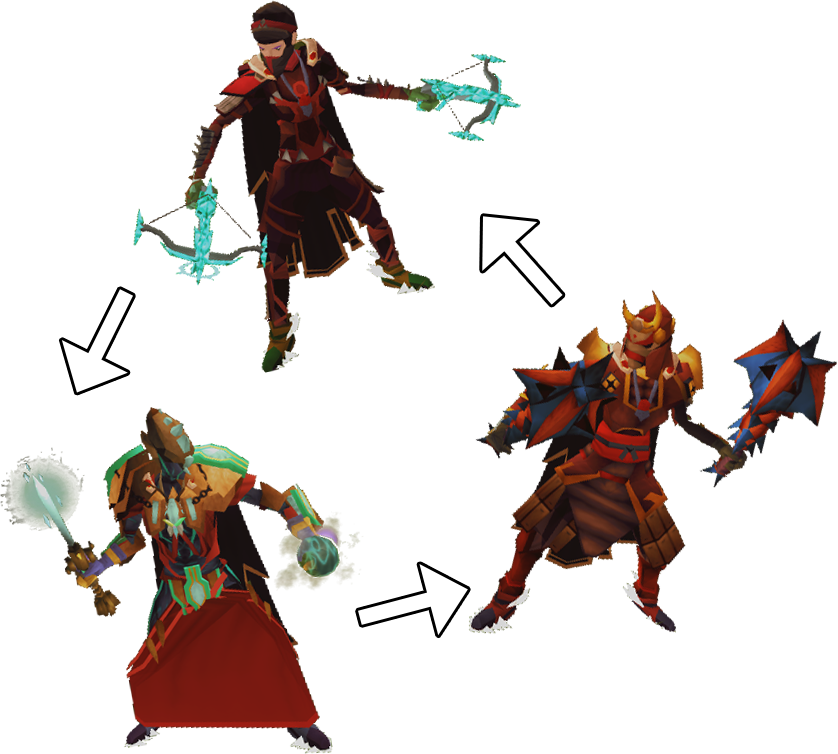
\includegraphics[width=.5\linewidth]{figures/runescape_triangle.png}
	\caption{The combat triangle for the game RuneScape.\cite{wiki-runescapecombat}}
\end{figure}

The other job, cleric, is not part of the combat triangle. As a supporting character class, we want it to have this following conflicting characteristics: (1) clerics should be weak attackers, but (2) the healing ability the job provides make parties with clerics stronger than those without. The contrast between individual weakness against group strength suggests that a balance is also required here. This is our secondary objective -- balancing the clerics against the other three attacking-type jobs.

Note that the three black magic elements -- fire, water, and nature -- also form their own tactical rock-paper-scissors. However to limit the level of complexity it will not be included as an objective.

\subsection{Battle system evaluation}
\label{sub:battleeval}

\subsubsection*{Evaluate a single constraint}

The method of evaluation depends on the objectives. For the combat triangle, we propose the following method of evaluation:
\begin{itemize}
\item Given two jobs, define a \textit{target win rate} as a number between 0 and 1. This is the target probability that the first job would win against the second on a random battle.
\item Simulate a number of random battles between the two jobs. First create two parties, one consists only of random units with the first job, and another with the second job. Then use the AI player to control the actions of both parties.
\item Count the number of times the first job wins the battle, and compare against the target win rate. The closer the actual win rate is to the target, the better.
\end{itemize}

The result of this method can be quantified by the \textit{objective function}, defined as the absolute difference between the actual win rate and the target win rate. The goal is then to minimise this function. We defined the target win rate as $0.8$ for all the advantages in the combat triangle.

As for the clerics-as-supporting-characters objective, the following targets are used:
\begin{itemize}

\item The win rate for a party with no clerics, against a party of clerics only, is set to 0.9 -- almost always. 
\item The win rate for a party with exactly one cleric, against a party with no clerics, is set to 0.7 -- a sizeable amount of advantage that is not too strong.
\end{itemize}

With a slight modification, the same evaluation method can also be used on this objective as well. Instead of specifying two jobs, two sets of \textit{job quotas} -- the exact number of units with the associated job -- are needed. All required constraints can be described in this way. For example, a party with exactly one cleric has a quota \texttt{[clerics = 1]}; an all-cleric party has quotas \texttt{[warriors = 0]}, \texttt{[rangers = 0]}, and \texttt{[mages = 0]}.

An implication of specifying objectives in this way is that the implementation would need to be able to support this kind of constraints upon instantiating battles.

\subsubsection*{Combining objectives}

If there is a single objective, then comparing battle systems is straightforward -- given our method of evaluation, the system that evaluate to the lowest value is the best. However there are already two major objectives -- the combat triangle and the clerics as helpful supporters. It is then not obvious how to compare these numerical values.

A sensible approach is to combined them into a single value. Researches in this area have offered a number of methods to achieve this task, as summarised in \cite{marler2004survey}. Some easy-to-implement options are min-max method, weighted sum, and weighted product. The optimisation process will need to experiment with these options to find out which gives the best result.

\section{The AI player}
\label{sub:aidesign}

The evaluation process we have laid out is based on the concept of \textit{self-play} -- simulating a number of battles using the same AI. The more competent the AI is, the better the evaluation.

The ultimate objective of the AI is to maximise its chance to win the battle. If the exact win probability is known for every possible instance of the battle, then the AI can simply choose the move that ends in the situation with the highest win probability. Unfortunately, that is not the case, as the exact win probability is difficult, if not impossible, to compute. Instead, we will use a heuristic based on the potential of each action to affect the amount of HP in the favourable direction to the AI's party.

Here we introduce the concept of \textit{HP-change potential}, which is a property of each possible action applied on a target unit. The actions are limited to the sensible ones: making damage to the enemies and healing units in the same party. The potential is defined as:
\[
	\Delta HP \times R^M
\]
where $\Delta HP$ is the expected change to HP (expected damage or expected recovery, as appropriate), $R$ is a discount coefficient between 0 and 1, and $M$ is the minimum number of moves required for the action taker to be able to execute the action.

The heuristic can be outlined as follows. First, the AI considers all its choices of action that can be done within this turn -- those which are immediately possible from the unit's current position, and those that are possible after moving the unit one time. It then finds the actions whose expected resulting effect would be largest, in terms of HP, i.e. the action with largest HP-change potential. If such an action exists, then:
\begin{itemize}
	\item If it can be executed immediately, then the AI would do it.
	\item If it requires a move, then the AI would move to one of the positions that allows it to make the action, then execute the action.
\end{itemize}

In the first case above, and in the case that no actions can be made, the unit would still have a free move that can be used to gain more advantage. In the second case, if there are multiple positions that allow the execution, then the AI should also choose the best among them. Choosing the best positions is done by considering the potential of each cell, from the following components:
\begin{itemize}
	\item $p_1$: the maximum HP-change potential the current unit can do from that position.
	\item $p_2$: The sum of all healing-type HP-change potential that all friendly units can do to the current unit, if it is in that position.
	\item $p_3$: The sum of all attacking-type HP-change potential that all enemy units can do to the current unit, if it is in that position.
\end{itemize}
The weighted sum $w_1 \cdot p_1 + w_2 \cdot p_2 - w_3 \cdot p_3$ is taken as the cell potential. All the weights should be configurable.

With this information, the `best move' is then easily defined, as the move to the cell with the highest cell potential.

\section{Battle system optimisation}

There are several optimisation techniques that might be applied to this task. One natural method that has been used in similar situations is \textit{genetic algorithm} (GA). GA is essentially a search-based technique. It systematically generates new solutions by maintaining a \textit{population} of possible solutions, which are initialised randomly, and try to create better solutions using the principle of natural selection, adopted from evolution in nature. The process prefers `fitter' members of the population -- those that give better evaluation result -- to survive and produce the next generation. Some of the weaker members also have some chance to survive in order to maintain variety in the population, as using only fitter members could quickly and easily leads to stagnation -- a local minimum. After a termination condition is fulfilled, the fittest member of the population is declared the best solution.

\section{Summary}

In this chapter the solution has been fully designed. The model and rules of the battle was laid out, and the configurable parts of the model was extracted out as the battle system. Basic requirements for the user interface was also described. We described how a reasonably competent AI player could be constructed, and how it would help in evaluating the battle system. Finally we proposed to use genetic algorithm as the strategy to arrive at a good battle system.
\chapter{Implementation}

The solution, according to the design from the previous chapter, consists of a number of interacting components. To eliminate any possible issues that might happen from integration, all the components were implemented using the same programming language -- Java 8. The solution would be built as a single executable \texttt{.jar} file, with all components bundled into it.

Development was done incrementally -- at the end of each phase the solution would be in a state where it is a working (but incomplete) product on its own. First of all, the battle model was created, with a GUI to test it out. On top of that the AI player was developed. Genetic algorithm can then be applied to optimise the battle systems. Finally, after some adjustments, the solution was adapted into a form suitable for human volunteers to evaluate the resulting battle system.

\section{Phase \rom{1}: manually-controlled battle}

The purpose of the first phase is to build a completely playable game, which requires the complete battle model, the battle controller, and a GUI.

\subsection{Model classes}

Central to the solution is the battle model. The entity classes were put into package \texttt{models} and its subpackage. Relationship among major entity classes are shown in figure \ref{fig:uml_models}.

\begin{figure}
	\centering
	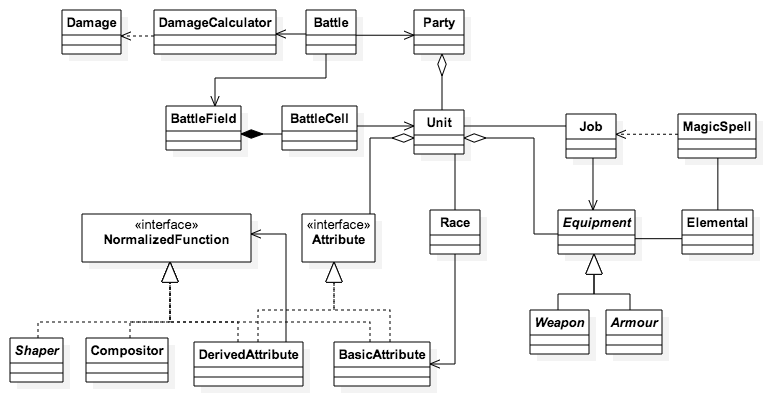
\includegraphics[width=1\linewidth]{figures/uml_models.png}
	\caption{Entity relationship for important model classes.}
	\label{fig:uml_models}
\end{figure}

A subpackage contains parts of the model with sufficient complexity to justify its existence. Notable ones are \texttt{models.equipment}, which contains the models for all weapons and armours, and \texttt{models.calculation} which describes the numerical derivation part of the combat rules.

\subsection{Preliminary battle system}

In this first phase it was not yet necessary to create the full-scale battle system. The calculation, which would later be extracted and parameterised into the battle system, was all fixed at this stage. A few adjustments to the calculation were done manually, just enough to keep the battles from being extremely unbalanced.

As for the derivation functions that map basic attributes to derived attributes, they were also arbitrarily fixed to be one of the following simple shaping functions:
\begin{itemize}
	\item Linear function $f(x) = x$.
	\item Quadratic function $f(x) = x^2$.
	\item Square root function $f(x) = \sqrt{x}$.
	\item The normalized logistic function $f(k, x) = \frac{k^{2x}-1}{(k-1) \cdot (k^{2x-1} + 1)}$, with $k = 10$.\footnote{$f(k, x)$ describes a set of functions $f(x)$ that are results of shifting the logistic function $\frac{1}{1 + e^{-x}}$ to pass through all of the points $(0, 0)$, $(0.5, 0.5)$, and $(1, 1)$.}
\end{itemize}

The battle system would be revisited in phase \rom{3}, where we made it fully configurable.

\subsection{Battle controller}

The battle controller is the centre of communication of the system. The class \texttt{BattleController} implements the behaviour specified in section \ref{sub:battlecontroller} faithfully for the most parts. We made one modification, by adding a loop-breaking condition to the main game loop (previously the game ends only when one side wins). This condition is defined based on the number of turns played in the battle. With this loop-breaking condition, battles that go on for too long can be cut short and declared as being tied. This is to prevent the game from getting stuck in an infinite loop, which could happen in an AI-vs-AI battle that has fallen into an equilibrium.

The battle controller keeps track of the position and timing of all the units. It maintains a \textit{priority queue} that sorts the units by their \textit{action time}, in ascending order. The action time tells when is the next time the unit will get its turn. At the start of the battle, the action time for each unit is initialised to its \textit{charge time} ($\frac{1}{\text{speed}}$). The controller then \textit{let the time progress}, and the unit with the least action time is then selected as the one who gets the next turn. Once the turn is finished, the unit is put back into the queue, with action time equal to the sum of the current time and its charge time.

The model defines an abstract type \texttt{Player}, which has an abstract method \texttt{selectPlay(Unit, List<CommandType>)} that encapsulates the play-selection strategy for each concrete implementation. The controller repeatedly asks the current player to provide the battle actions, updates the battle model accordingly, then notifies the UI and any other interested components about the change.

As stated in the design stage, the notification mechanism was implemented as an event-driven system. We utilised \textit{EventBus}, an annotation-based event handling library which is a part of Google's \textit{Guava} utilities, to do this task. On the event poster side, the following events are posted when triggered by their associated actions:
\begin{itemize}
	\item \texttt{UnitActionEvent}: tells subscribers that a unit has completed an action.
	\item \texttt{DamageEvent}: tells subscribers that an action that can cause damage (including healing -- for convenience we can think of healing as a \textit{negative damage}) is attempted on a unit, successfully or not.
	\item \texttt{UnitDeadEvent}: tells subscribers that a unit is removed from the battle.
	\item \texttt{BattleEndEvent}: tells subscribers that the battle has ended.
	\item \texttt{ActionTargetAreaEvent}: informs subscribers about \textit{target area} -- the set of all possible target cells of a command. For example, when the player chooses the \textit{move} command, this event will tell subscribers about all possible cells that can be the destination of the move.
\end{itemize}

Notice that a single action can cause multiple events. An attack command would generate at least three events, definitely one each of \texttt{UnitActionEvent}, \texttt{DamageEvent}, and \texttt{ActionTargetAreaEvent}. If the attack kills the target then a \texttt{UnitDeadEvent} is also generated. Even a  \texttt{BattleEndEvent} is possible, if the attack kills the last opponent.

\subsection{Random battle generator}

To start a battle, all the pieces of the model need to be instantiated and assembled together. In this phase we only focused on generating random battlefields in a systematic way, whereas everything else was created simply by random selection from finite options.

The design states that the battlefield must be generated in a way that all accessible cells are connected. We added another constraint here: there must be at least 4 accessible cells in the two topmost rows, and at least 4 accessible cells in the two bottommost rows. This is because we want to put the two parties on these rows at the start of the battle, one at the top and the other at the bottom, similar to the starting configurations in chess or checkers. 4 is the maximum number of units in party we used, so at least 4 empty, accessible cells are needed for each party.

The algorithm used to create the battlefield is a variant of the flood-fill algorithm:
\begin{enumerate}
	\item Start with an empty battlefield. Mark the \textit{middle} cell $(\frac{width}{2}, \frac{height}{2})$ as accessible, with an initial height $h_0$. Add the 4 cells adjacent to this middle cell to the \textit{fringe} set.
	\item Randomly select one cell $c$ from the fringe.
	\begin{enumerate}
		\item Mark $c$ as accessible.
		\item Find the set of cells adjacent to $c$ that have already been marked as accessible (at least one exists, otherwise $c$ would not be in the fringe). Randomly pick one of these, and call it $s$.
		\item Set the height of $c$ to either $h_s-1$, $h_s$, or $h_s+1$, where $h_s$ is the height of $s$.
		\item Add all cells adjacent to $c$ that has not been marked as accessible to the fringe.
	\end{enumerate}
	\item Repeat the previous step until the desirable number of accessible cells is reached.
	\item If the number of accessible cells in the two topmost rows or in the two bottommost rows is less than 4, redo the whole process from the beginning.
\end{enumerate}

In simple terms, the algorithm starts from a set of one accessible cell, then repeatedly, randomly expands this set, while maintaining the total-connectedness of all accessible cells.

\subsection{User interface}

\begin{figure}
	\centering
	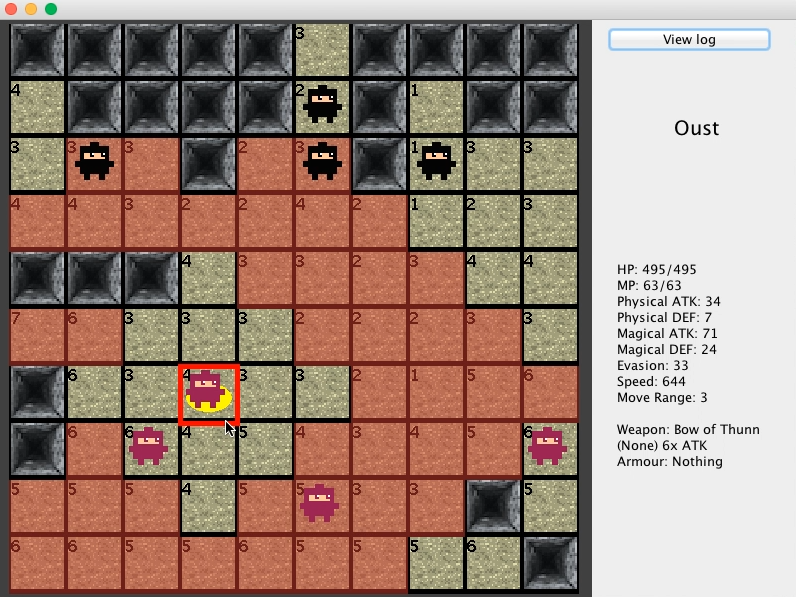
\includegraphics[width=.8\linewidth]{figures/battle1}
	\caption{Battle GUI during phase \rom{1}.}
	\label{fig:guiphase1}
\end{figure}

In this phase, a graphical user interface was implemented as a single-screen Java Swing application, as shown in figure \ref{fig:guiphase1}. This simple GUI allows the battle mechanics to be manually tested. It has the following features:
\begin{itemize}
	\item It displays the battlefield as a 2-D rectangular grid. Accessible and inaccessible cells are distinguished using different background patterns. The height of each accessible cell is written at the top.
	\item Units are displayed on the battlefield using the same sprite, distinguished only by their colours (black or red), to indicate different parties.
	\item Hovering the mouse over a unit will display its statistics (including those of its equipment) in a panel on the right.
	\item A yellow oval is used to indicate the current unit. Clicking on this unit will pop up a menu where battle actions can be selected.
	\item When selecting actions that require a target cell, the eligible cells will be overlaid with a translucent colour (green for move command, red for battle commands). Clicking on one of these cells will commit the command, while clicking outside will cancel.
	\item A log of all actions in the current battle can be viewed by clicking on the \textit{View log} button.
\end{itemize}

For the task of finding the eligible cells, which is not required given the rules of the battle, nevertheless necessary for user experience, the following algorithm is used. It is another variant of breadth-first-search, flood fill algorithm:

Given a starting cell $o$, an adjacency test predicate $adj(c_1, c_2)$, a cost function $cost(c_1, c_2)$, and a maximum cost $C$. 
\begin{enumerate}
	\item Initialise a queue with the starting cell.
	\item Initialise a map $M$ to record the cost of each eligible cell. Set $M[o] = 0$.
	\item Repeat until the queue is empty:
	\begin{enumerate}
		\item Take a cell $x$ out of the queue.
		\item For each cell adjacent to this cell (that is, for every cell $y$ passing the adjacency test $adj(x, y)$), calculate the new cost $nc = M[x] + cost(x, y)$.\footnote{The cost function is usually a uniform function $cost(x, y) = 1$, but different scheme can be applied if the game rule changes.}
		\item If $nc$ is greater than the maximum cost $C$, ignore this cell.
		\item If $M[y]$ is not recorded yet, or if $nc < M[y]$, then set $M[y] = nc$ and put the cell $y$ into the queue. 
	\end{enumerate}
	\item All the keys in the map $M$ are the resulting eligible cells.
\end{enumerate}

\bigskip
At the end of this phase, the program was in a playable state, with random battlefield and units each time a battle was generated. The game was in 2-player mode since the AI did not exist yet. We had no control over how the units were generated, and the battles could be quite overpowered at times, since the mages were very weak in this system. These missing components would be created in later phases.

\section{Phase \rom{2}: automated player}

In this phase, the AI player was introduced. It was implemented as a concrete subclass of \texttt{Player}, called \texttt{SmartPlayer}. It follows the concept of \textit{HP-change potential}, as described in the design in section \ref{sub:aidesign}. Although the strategy involves complex calculation steps, the implementation itself follows the design rather straightforwardly. 

The basic building block of the strategy is the amount of damage (and healing) when a unit makes a certain combat action against a target. Damage calculation, as described in section \ref{sub:dmgcalc}, includes a random variation that makes the actual amount of damage varying in the range of 50\% to 150\% of the base damage. It is also possible for an action to be unsuccessful, depending on the \textit{evasion} attribute of the target. These two factors make the exact amount of damage uncertain. We could have programmed the AI and the battle model in such a way that the AI is an \textit{omniscient agent} -- i.e.\ having full access to the exact outcome of any actions.\cite{russell2010artificial} However it was decided that that would give the AI too much unfair advantage, and the AI should only be allowed to know what can be theoretically known to human players -- which obviously do not include results of randomisation. Instead the AI uses the \textit{expected damage}, calculated simply as the \textit{product of the base damage and the chance of success}, which is $(1 - \text{target's evasion})$. 

The strategy also includes finding the number of moves required for a unit to attack another. There would be a lot of redundant calculations if this is implemented naïvely. Therefore, a cache of the distances (in terms of number of moves required for each unit) between all pairs of battle cells is maintained. These distances are figured out only once using the flood-fill algorithm previously described. Once calculated, they can be reused throughout the battle, thus in the long run this improves the time-efficiency of the AI.

The GUI was extended to let the user select the two players, so the battle can be Human vs Human, Human vs AI, or AI vs AI. We observed the behaviour of the AI, given different values to the configurable weights of each sub-strategy (attacking, healing, or avoiding damage). We found that if avoiding-damage is given too much weight, battles could end as draws very easily, since both parties would prefer to maintain safe distance out of attacking range of the other. Therefore we calibrated the weights so that the AI prefers attacking a little more than healing, and avoiding damage is given very little weight, effectively acting as a tiebreaker only.

At this stage we tested the AI manually, by playing against it, and found that it was competent to a satisfactory degree. It did not make useless moves, and it was capable of winning against us quite often.

\section{Phase \rom{3}: procedural generation of balanced battle system}

In this phase, as we already had a stable battle model and AI, we turned our focus to the battle system development and generation.

\subsection{Full battle system}

The battle system is a collection of configurable parts of the model. In the first two phases, these were embedded throughout the model classes. It would be most convenient and manageable if all the configurations are aggregated together in the same module. The class \texttt{BattleSystem} was created for this purpose. It collects all the configurable parts as public, serializable fields.

As the plan is to eventually generating battle systems using genetic algorithm, the class has to be designed to work in conjunction with \textit{Jenetics}\cite{holzinger2014interactive}, the genetic algorithm framework we will use. Jenetics works on a population of \textit{genotypes} -- structural representatives of the solution -- in this case, a \texttt{BattleSystem} instance. A genotype consists of several \textit{chromosomes}, which in turns consist of several \textit{genes}. For simplicity we conflated the concepts of chromosomes and genes together, by fixing the number of genes per chromosome to 1. Each configuration value then needs to be expressed in terms of chromosomes.

Jenetics provides a few different data types that can be used as a chromosome, therefore a solution can be encoded not only as a \textit{bitstring}, but also as a sequence of integers or floating point numbers. The data type in a single genotype is required to be the same\cite[6]{jenetics-manual}, and we chose \textbf{integers} as the basic building blocks. All the configuration values identified from section \ref{sub:battlesystemdesign} can be classified into four groups:
\begin{itemize}
	\item integers
	\item floating point numbers
	\item derivation functions with a single source
	\item derivation functions with two sources
\end{itemize}
Each of these would need to be converted to one or more integers. Integers themselves obviously need no conversion. For floating point numbers, they are multiplied by 100 and rounded to the nearest integer, therefore preserving the original precision at the scale of 0.01. Derivation functions are more complicated.

\begin{figure}
	\centering
	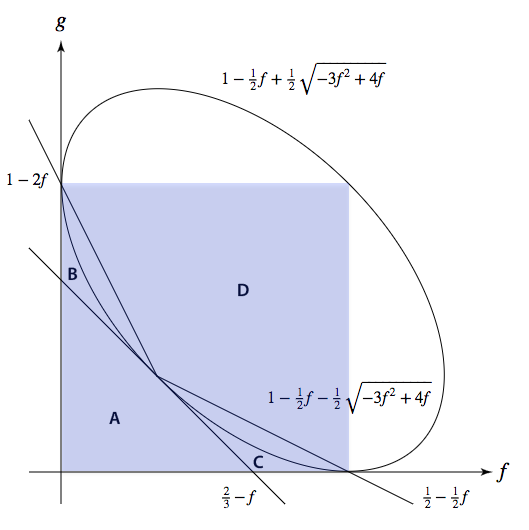
\includegraphics[width=0.7\linewidth]{figures/bezier}
	\caption{This graph shows the eligible area that the other two control points can be placed, when fixing the first and last control points to (0, 0) and (1, 1), that would preserve the monotonicity property of the Bézier curve. The purple square is the area within (0, 0) and (1, 1), which is completely inside the eligible area. (Graph adapted from \cite{web-bezier})}
	\label{fig:bezier}
\end{figure}

In phase \rom{1}, each derivation function was selected from a small set of functions. Here we wanted more flexibility, so \textit{cubic Bézier curves} were chosen in their place. Cubic Bézier curves are parametric curves with 4 control points, often used in computer graphics. They can also be used as shaping functions.\cite{web-flong} By fixing the first ccontrol point to the origin, the last control point to (1, 1), and the other two to be in the unit square, it can be guaranteed that the resulting curve will be a shaping function -- a monotonically increasing function that passes through (0, 0) and (1, 1).\cite{web-flong, web-bezier} Therefore the derivation functions with single source can be encoded as 4 floating points -- 2 points for each unfixed control point, plus another integer for maximum domain value. The floating point numbers are then converted to integers, resulting in 5 integer parameters per derivation function. Derivation functions with two sources use similar conversion process, with another floating point parameter for the weight given to the first source, resulting in 6 parameters per function.

Using the process as outlined above, a battle system can be encoded as a genotype of 96 integers.

\subsection{Battle generator and constraints}

Evaluation of battle systems requires simulating battles in some constrained environment. In this phase the battle generator was extended by allowing constraints to be specified on the units to be generated.

Aside from the battlefield generator which was implemented in phase \rom{1}, the following capabilities were added:
\begin{itemize}
	\item The basic attributes of each unit are still generated randomly, but the average and maximum deviation of these values can be set. The default setup values we used are 0.5 for the average and 0.3 for the deviation, which allow the range of attributes to be [0.2, 0.8].
	\item The material attributes of each equipment can also be constrained in the same way.
	\item The number of units with specific job types can be constrained, using the quota system as described in section \ref{sub:battleeval}.
	\item Races can also be constrained in the same way.
	\item Equipment types are constrained indirectly by the choice of jobs.
	\item A generator can be serialized to a JSON data file.
	\item The whole process is deterministic, meaning that given the same configuration and random seed, the end result will also be exactly the same.
\end{itemize}

The implementation of these features are located in the subpackage \texttt{generators} and \texttt{generators.constraints}.

\subsection{Evaluator and the combined objective}

In the design stage, two major objectives were stated: the combat triangle and the clerics as helpful supporters. We have also added a simple objective named `no first-mover advantage', stating that both parties should have equal chance of winning a random battle. All of these are based on the same principle of evaluation: they were all measurements of win rate for a given situation.

The evaluator takes a battle system and evaluates it against a given objective, with a specified method of combination. The objective would reference all the necessary battle generators. For each generator, AI self-battles will be simulated for a given number of times. The following are collected, by listening to the events issued by the controller:
\begin{itemize}
	\item Raw statistics for each generator, such as the winning percentage of the first team against the second, total runtime, or the average number of turns in a battle.
	\item The fitness of all the objectives at every level.
\end{itemize}

To combine multiple fitness values $V = \{v_1, v_2, \ldots, v_n\}$ together, given weights $w_1, w_2, \ldots, w_n$, and $W = \sum_{i=0}^{n} w_i$, the following options of combination were implemented:
\begin{enumerate}
	\item \textbf{Min-max method}. As our objective is to minimising, this method would simply takes $\min(V)$ as the combined objective. This method ignores the weights.
	\item \textbf{Weighted average}. The combined objective is $\frac{\sum_{i=0}^{n} w_i \cdot v_i}{W}$.
	\item \textbf{Weighted geometric mean}. The combined objective is $  \sqrt[\uproot{3}W]{ \prod_{i=0}^{n} v_i^{w_i}}$.
	\item \textbf{Weighted-normalised geometric mean}. This is similar to the regular weighted geometric mean method, but each sub-objective is added by 1 before taking the geometric mean, to handle the case where one sub-objective has a value of zero, which would render all other sub-objectives irrelevant. The combined objective is then $\sqrt[\uproot{3}W]{ \prod_{i=0}^{n} (v_i + 1)^{w_i}}$.
\end{enumerate}

The evaluator was implemented as both a routine that can be called from another class -- intended to be used by the procedural generation process, and as a command line program.

\subsection{Procedural generation by genetic algorithm}

As planned from the design stage, battle systems are procedurally generated using genetic algorithm. We utilised \textit{Jenetics}, a genetic algorithm framework implemented using the stream concept of Java 8 that promotes parallelization.

The process works as follows:
\begin{enumerate}
	\item A starting \textit{population} of candidate battle systems is created, either from random \textit{genotypes}, or from existing population from a previous run.
	\item Each member of the population is evaluated, using a \textit{fitness function} that calls upon the evaluator.
	\item Standard genetic algorithm operations (selection, crossover, mutation) are applied here to create the next generation of population from the current one. We used the following setup:\footnote{For details of these operations, see the Jenetics manual \cite{jenetics-manual}.}
	\begin{itemize}
		\item \textit{Tournament selection} of size 4 was used for survivors selection. The winner of a round-robin comparison between 4 randomly selected members survives.
		\item Offspring selection was also done using tournament selection, but the tournament size is 3 to reduce the selection pressure. The selected offsprings are then altered, using single-point crossover (swapping two genotypes at a single point) and Gaussian mutator (change a random gene within a genotype to a nearby number).
		\item The survivors and offsprings are combined to form the new generation.
	\end{itemize} 
	\item Repeat steps 2--3 until no improvement has been made for a fixed number of generations.
\end{enumerate}

Since each invocation of the fitness function performs a lot of computation, mainly on the simulation of AI self-battles, it is desirable for the evaluation to be done concurrently, to speed up the process. Jenetics does this by default, using Java's \texttt{ForkJoinPool.commonPool()}, which is considered to be appropriate in most cases.\cite{jenetics-manual} As long as the fitness function is implemented in a thread-safe manner then we can utilise this default setting without any intervention.

Even with multithreading, it still usually took several hours to complete the process from scratch. The evaluation procedure we eventually settled on works like this: the initial run would start from random population using min-max combinator, then the result of this run would be used as starting population for other combinators. This shortened the computation time needed, since the starting point for other methods is usually already producing a good outcome. The result battle system from each combinators are then compared, rather subjectively from game-playing experience, to evaluate which one works best.

\section{Phase \rom{4}: fine-tuning}

The implementation from the previous phase was complete, according to the design. But after running the genetic algorithm engine, it was found that the design was underspecified, and some more work is needed to make the system perform better.

\subsection{The overpowered system}

The first few attempts at generating battle systems produced very good results, measured against the objectives, especially the combat triangle objective. However, after playing those system manually, it was quickly found out that the battles under these systems were extremely short. Most of the attacks were either so powerful the target was killed instantly, or so ineffective that no damage was taken. While these systems are balanced, they are also too overpowered to the degree that the game was unplayable.

The first attempt to remedy this situation was to introduce a new objective that specifies a preference for the length of the game in terms of \textit{total number of turns}, by specifying a target number and evaluate battles to be better when the actual number of turns is closer to the target. More formally, we wanted to minimise the objective function $\frac{|n-t|}{t}$, where $n$ is the actual number of turns and $t$ is the target. It was found that this objective is very difficult to achieve, since all the target values we tried produce results with higher value than the combat triangle objective, as shown in figure \ref{fig:plot_multiobj}.
This objective was then abandoned.

\begin{figure}
	\centering
	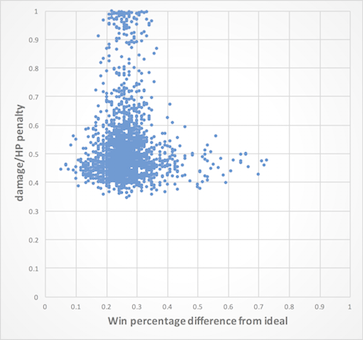
\includegraphics[width=0.6\linewidth]{figures/plot1}
	\caption{A plot of combat triangle evaluation ($x$-axis) against number-of-turn evaluation ($y$-axis), for every individual in all generations of a GA run. The $y$-value plateaus at around 0.35.}
	\label{fig:plot_multiobj}
\end{figure}

The second attempt was to use another objective function based on the size of damage. Damages are classified into 10 bins, based on their relative size to the maximum HP of the target unit, from 0\%-10\%, 10\%-20\%, and so on. Each bin has an associated \textit{penalty} value between 0  and 1, the lower indicating more desirable range of damage. The objective was set up to drive the damage into 10\%-40\% range. We found that this was better than the first attempt, but still difficult to achieve.

It was then suspected that the damage calculation might be too stiff, making it too difficult to optimise. As a result, more parameters were added specifically for this, generalising the \textit{base damage} calculation equation from:
\[
ATK \cdot \frac{ATK}{ATK+DEF}
\]
to:
\[
C_1 \cdot ATK^{C_2} \cdot (\frac{ATK}{ATK+DEF})^{C_3}
\]
The constants $C_1$, $C_2$, and $C_3$ improved the result, but still not to our satisfaction.

The last modification made was on the data collection method, where the percentage calculation was changed from:
\[
\frac{\text{actual damage}}{\text{max HP of the target}}\] to: 
\[
\frac{\text{actual damage}}{\text{average max HP of all units}}
\]
This makes the objective more focused, and easier to achieve. The resulting battle systems are no longer overpowered, while keeping the combat triangle intact.

\subsection{The ineffective black magic system}

Another unexpected result was from a battle system that is well-balanced in terms of the combat triangle, but black magic is surprisingly very weak. Mages do have strong advantage over warriors as specified in the objective, but not as a result of powerful magical attack. This was because the genetic algorithm had adjusted mages' physical attack to be very strong, while totally ignored black magic.

This is not a fault of the genetic algorithm, but rather because the constraints on the system are underspecified. There are implicit constraints that we failed to make explicit. In this case we should have specify that mages should not be able to do more physical damage than magical, or that the physical strength of mages should be less than other classes.

In any cases, the implementation do not have a mechanism to support these constraints, therefore a workaround was used instead: the AI was made to prefer magical over physical attack. At first we simply adjusted the weight of black magic, from about the same as physical attack, to twice higher. This was not effective, and we kept on increasing the weight, to no success. Finally we had to made adjustments to the AI implementation, so that whenever both black magic and physical attack are available, the AI will always choose the former. This solved the problem, so that the solution can produce battle systems that has combat triangle, and the strength of mages are from magical attack.

\subsection{Objective refinement}

Previously in this phase, another objective, the damage percentage, was added. We also realised that the combat triangle and the clerics objective are actually composed of multiple sub-objectives themselves, and the combination method was fixed to unweighted average for both. After this realisation, we had to go back and make radical changes to the implementation. Instead of being flat, single-levelled, objectives are now implemented as a tree-like recursive structure, where a single objective can be either atomic, or composed of other sub-objectives, as depicted in figure \ref{fig:objective_uml}. An objective tree can also be serialize to a JSON file. The final version of our objective tree is shown in figure \ref{fig:objectivetree}.

\begin{figure}
	\centering
	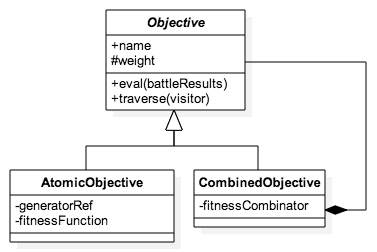
\includegraphics[width=0.7\linewidth]{figures/uml_objectives.png}
	\caption{The classes implementing the recursive objective structure.}
	\label{fig:objective_uml}
\end{figure}

\begin{figure}
	\centering
	\includegraphics[width=1.0\linewidth]{figures/objective_tree.png}
	\caption{The objective tree}
	\label{fig:objectivetree}
\end{figure}

The evaluation command was also adapted and improved as a result of this change. Previously, each sub-objective might refer to the same battle generator (since they share the same battle constraints), and each would generate and simulate the battles separately. This was redundant -- a single round of simulation would be enough for all these sub-objectives to get the necessary information. With this refinement, we had a chance to improve this process, by first collect all the battle generators, run each generator for only a single round, then notify the sub-objectives accordingly.

The objective combinator can be specified for each non-atomic node in the tree. From our subjective evaluation, the min-max combinator works much better than the original unweighted-average to combine the sub-objectives of the combat triangle and the clerics-as-supporters. At the root node we could not clearly identify the best combinator, so we settled for the min-max method as default, but this can be easily overridden from the command line.

\section{Phase \rom{5}: preparation for evaluation}

At the end of the previous phase, the solution could systematically produce battle systems that meet the specified objectives to a satisfactory degree. The next step is to let real players verify that they get the sense of balance from the generated system. The solution needs a few adjustments to prepare for this evaluation step.

\subsection{Recovery of the preliminary battle system}
\label{sub:recovery}

We want to compare the generated system, which is supposed to be well balanced, to another one that is not so. One choice of such other system is the preliminary battle system used back in phase \rom{1}. The implementation of the derivation function had changed a lot from that point -- the fixed set of functions were replaced by cubic Bézier curves. To recover the original system for use in evaluation, Bézier curves that approximate each of the original functions are required. By using numerical methods, the control points in table \ref{table:control_points} (figure \ref{fig:control_points}) were discovered as the ones that provide good approximation, and so the original system was recovered.

\begin{table}
	\begin{tabu}{X[l1] X[c1] X[c1] }
		\toprule
		function & $P_1$ & $P_2$\\ 
		\midrule
		Linear & $(0.5, 0.5)$ & $(0.5, 0.5)$\\
		Quadratic & $(0.333, 0)$ & $(0.667, 0.333)$\\
		Square root & $(0, 0.333)$ & $(0.333, 0.667)$\\
		Logistic & $(0.430, 0.196)$ & $(0.570, 0.804)$\\
		\bottomrule
	\end{tabu}
	\caption{Control points that approximate simple shaping functions}
	\label{table:control_points}
\end{table}

\begin{figure}
	\centering
	\begin{subfigure}{0.24\textwidth}
		\centering
		
\includegraphics[width=1\linewidth]{figures/approx_linear}
		\caption{Linear}
	\end{subfigure}
	\begin{subfigure}{0.24\textwidth}
		\centering
		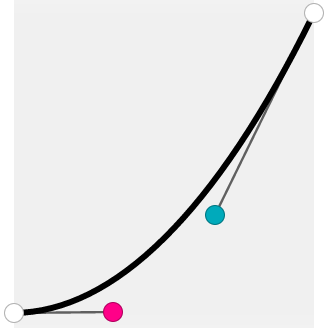
\includegraphics[width=1\linewidth]{figures/approx_quad}
		\caption{Quadratic}
	\end{subfigure}
	\begin{subfigure}{0.24\textwidth}
		\centering
		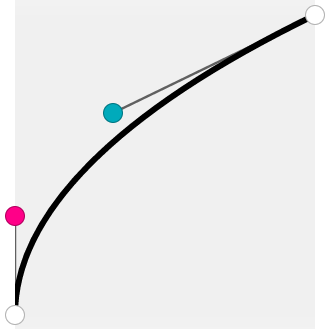
\includegraphics[width=1\linewidth]{figures/approx_root}
		\caption{Square root}
	\end{subfigure}
	\begin{subfigure}{0.24\textwidth}
		\centering
		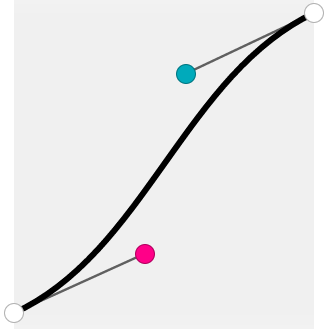
\includegraphics[width=1\linewidth]{figures/approx_S10}
		\caption{Logistic}
	\end{subfigure}
	\caption{Control points and the shape of each approximation of simple shaping functions}
	\label{fig:control_points}
\end{figure}

\subsection{GUI extension}
\label{sub:guiextension}

The GUI had to be extended to accommodate the evaluation process. The following changes/extensions were made:

\begin{figure}
	\centering
	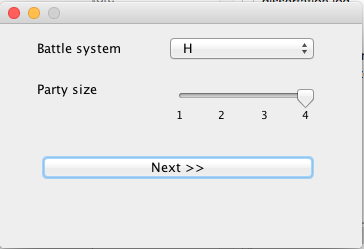
\includegraphics[width=.36\linewidth]{figures/gui_first}
	\caption{Battle system and party size selection screen}
	\label{fig:gui1}
\end{figure}

\begin{figure}
	\centering
	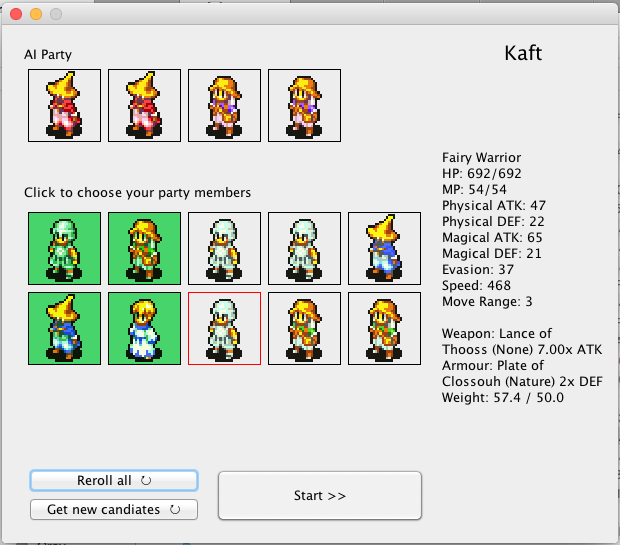
\includegraphics[width=.62\linewidth]{figures/gui_selector}
	\caption{Party selection screen}
	\label{fig:gui2}
\end{figure}

\begin{figure}
	\centering
	
	\begin{subfigure}{1\textwidth}
		\centering
		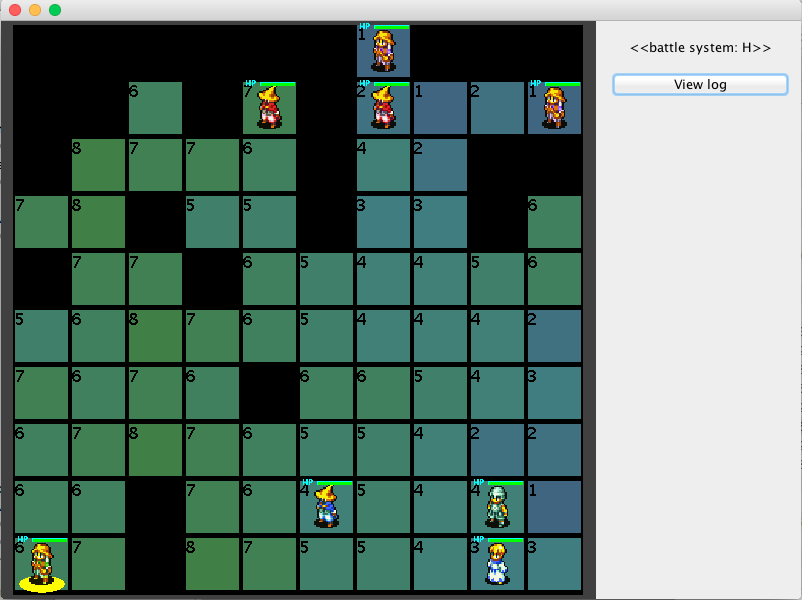
\includegraphics[width=.9\linewidth]{figures/gui_start}
		\caption{At the start of the battle}
	\end{subfigure}
	
	\begin{subfigure}{1\textwidth}
		\centering
		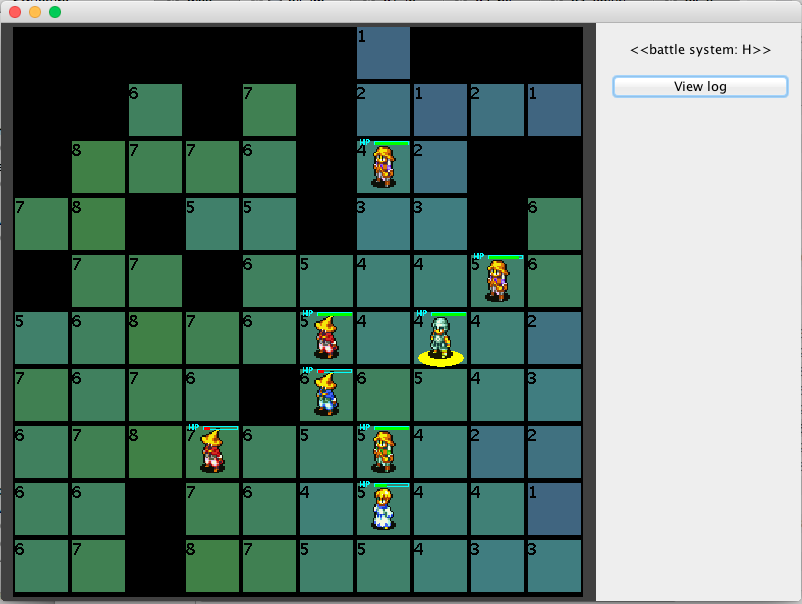
\includegraphics[width=.9\linewidth]{figures/gui_midgame}
		\caption{At the middle of the battle}
	\end{subfigure}
	\caption{Battle screen}
	\label{fig:gui3}
\end{figure}

\begin{itemize}
	\item The interface now consists of three main screens. The first one (figure \ref{fig:gui1}) asks users to pick a battle system and size of the parties.
	\item The second screen (figure \ref{fig:gui2}) shows the AI's party, and 10 units that users can pick to form their party. If the available options are not satisfactory, the users can also hit `reroll' to get a new set of candidates.
	\item The third screen (figure \ref{fig:gui3}) shows the battle, with improved graphical displays. The colour of each cells now provides visual clue to its height. The unit sprites\footnote{The sprites are from the game \textit{Final Fantasy Tactics}. All rights belong to Square Enix.} were changed to make it easier to distinguish between different jobs. There is also an HP bar above each unit, showing its current HP.
\end{itemize}

These changes were mostly small extensions on top of the existing solution. The only exception is the party selection mechanism, which requires generating more units than the party size, thus the battle generator had to be modified. Also, the flow of the program allows users to quit the battle, come back to the party selection, change the members of the party and restart the battle. This raises an issue -- since we used the same model for the units in the selection process and in the battles, if the users quit, then restart the battle, stats like HP/MP that have already been reduced from the previous battle would not be refilled. This was solved by using different copies of the unit instances in the selection process and in the battle. The serialization framework \textit{Kryo} is used for this task, as it enables fast deep-cloning of custom Java objects.

\section{Testing}

Automated test cases were created to ensure the correctness of the implementation, but these are mostly focused on the \texttt{models} module, where most of the calculation happens. Code coverage (measured in terms of number of instructions) for each of the classes in these modules is at least 70\%, as seen in figure \ref{fig:coverage}.

\begin{figure}
	\centering
	
	\begin{subfigure}{1\textwidth}
		\centering
		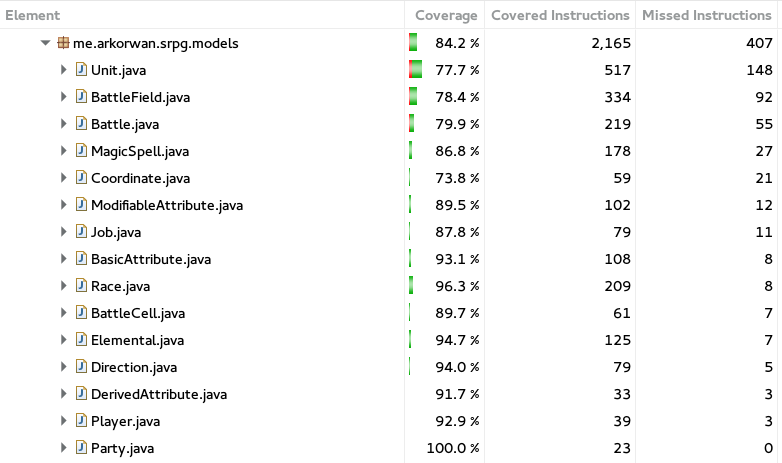
\includegraphics[width=.9\linewidth]{figures/coverage_models.png}
		\caption{The main \texttt{model} package}
	\end{subfigure}
	
	\begin{subfigure}{1\textwidth}
		\centering
		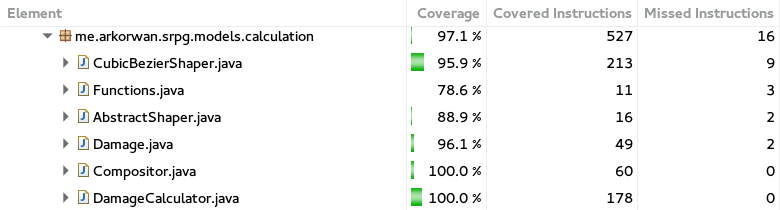
\includegraphics[width=.9\linewidth]{figures/coverage_calculations.png}
		\caption{The \texttt{calculation} subpackage}
	\end{subfigure}
	\caption{Code coverage}
	\label{fig:coverage}
\end{figure}

For other components, manual testing was applied. First, the GUI was manually, exploratively tested after phase \rom{1}, by playing multiple human vs human battles. The AI was tested after phase \rom{2}, by playing multiple human vs AI, and AI vs AI battles, and observing the progress of the game to make sure that the AI did not make any unreasonable choices. The evaluator and genetic algorithm engine were tested by actually run the genetic algorithm, rerun the evaluator on the resulting system to double-check that the results agree, then manually play the resulting system to see if the statistics agree with the actual gameplay.

\section{Challenges and issues}

Throughout the development process there were issues we have encountered. Some were already addressed in phase \rom{4} of the development. This section describes some other notable incidents.

\subsection{Consequences of using EventBus}

EventBus is used in our solution to provide event-based communication between the controller and the subscribers (GUI and the evaluator). It is a convenient solution, but our misuses had caused two related issues:
\begin{itemize}
	\item When an object wants to listen to events, it subscribes to an EventBus instance. The subscriber would then be back-referenced by the EventBus instance, keeping it in the memory until unregistration. One problem we encountered was a memory leak, first observed during the genetic algorithm process, which happened because we failed to unsubscribe evaluators that already finished their work. The leaked evaluator instances would eventually crash the process. The problem was difficult to identify, but easily fixed by adding proper unregistration.
	\item Another problem was that we used a single, centralised EventBus instance for all the battles. When there are multiple battles running concurrently, all the subscribers would get events from all the battles, thus the evaluators would collect more statistics than it should, leading to wrong results. This was fixed by making a dedicate EventBus instance for each battle.
\end{itemize}

\subsection{Deep-cloning of functional interfaces}

As a part of adapting the solution for the evaluation process, unit instances need to be deep-cloned. The serialization framework \textit{Kryo}\footnote{\url{https://github.com/EsotericSoftware/kryo}} is used for this task, as it enables fast deep-cloning of custom Java objects. Most of the elements in the object graph can be cloned without any special handling, except for the \texttt{Compositor} class, which is used to combined two shaper functions into one. This class has a field of type \texttt{DoubleBinaryOperator}, which is a functional interface type introduced in Java 8. Kryo did not handle it as well as other classes, throwing exception when trying to serialize these objects. To solve the problem, these steps have to be followed:
\begin{itemize}
	\item For the functional interface to be serialized (\texttt{DoubleBinaryOperator}), create a new interface (\texttt{SerializableOperator.Binary}) that extends both the original functional interface, and the \texttt{Serializable} interface. Replace the interface to be serialized with this newly created one.
	\item Register a special class to the serializer instance, as follows:
	\begin{lstlisting}[language=Java]
kryo.register(Class.forName("com.esotericsoftware.kryo.Kryo$Closure"), new com.esotericsoftware.kryo.serializers.ClosureSerializer());
	\end{lstlisting}
	The class has to be loaded dynamically by name, since it has been made private by mistake. This has been fixed, and would be included in the next Kryo release\footnote{See the pull request at \url{https://github.com/EsotericSoftware/kryo/pull/415}.}.
\end{itemize}

\section{Summary}

In this chapter, the solution was realised from the design to a concrete program. Most of the implementation sticks closely to the design, but there are some changes along the way, as unforeseen issues were encountered and resolved. At this stage we have a working program that can be used to produce a well-balanced battle system, the quality of which will be evaluated in the next chapter.
\chapter{Evaluation}

The solution is now in its completion. It can produce a battle system that,  according to itself, is well-balanced. In this chapter we will try to validate if humans agree with this claim or not.

\section{Evaluate a battle system for balance}

\subsection{Methodology}
\label{sub:meth}

In order to evaluate the solution, first we ran the solution to generate a battle system with balance as the objective. We then picked another system, evaluated to make sure that according to the same evaluation criteria, it was not as balanced as the generated one. Then we let human volunteers play the game on both systems, without telling them which one was generated, and asked them a series of questions to identify which system they thought was more balanced.

\subsubsection*{Balanced system}

To produce a balanced battle system, the genetic algorithm part of the solution was run, using the following configurations:
\begin{itemize}
	\item Population size is 50.
	\item Stop GA process after no better solution could be found for 30 generations. (Maximum generation is 500, but this is irrelevant.)
	\item Use min-max as the top-level fitness combinator, to combined the 4 major objectives.
	\item Simulate 50 battles for each matchup in each generated battle system.
	\item A battle ends as a draw if no clear winner emerges after 200 turns.
\end{itemize}

The process was run twice, producing two different `best' systems (because of inherent randomness in the GA process). The one with the lower fitness was chosen. Figure \ref{fig:systemj} shows the entire run that produced this system, with the best fitness of 0.2.

\begin{figure}
	\centering
	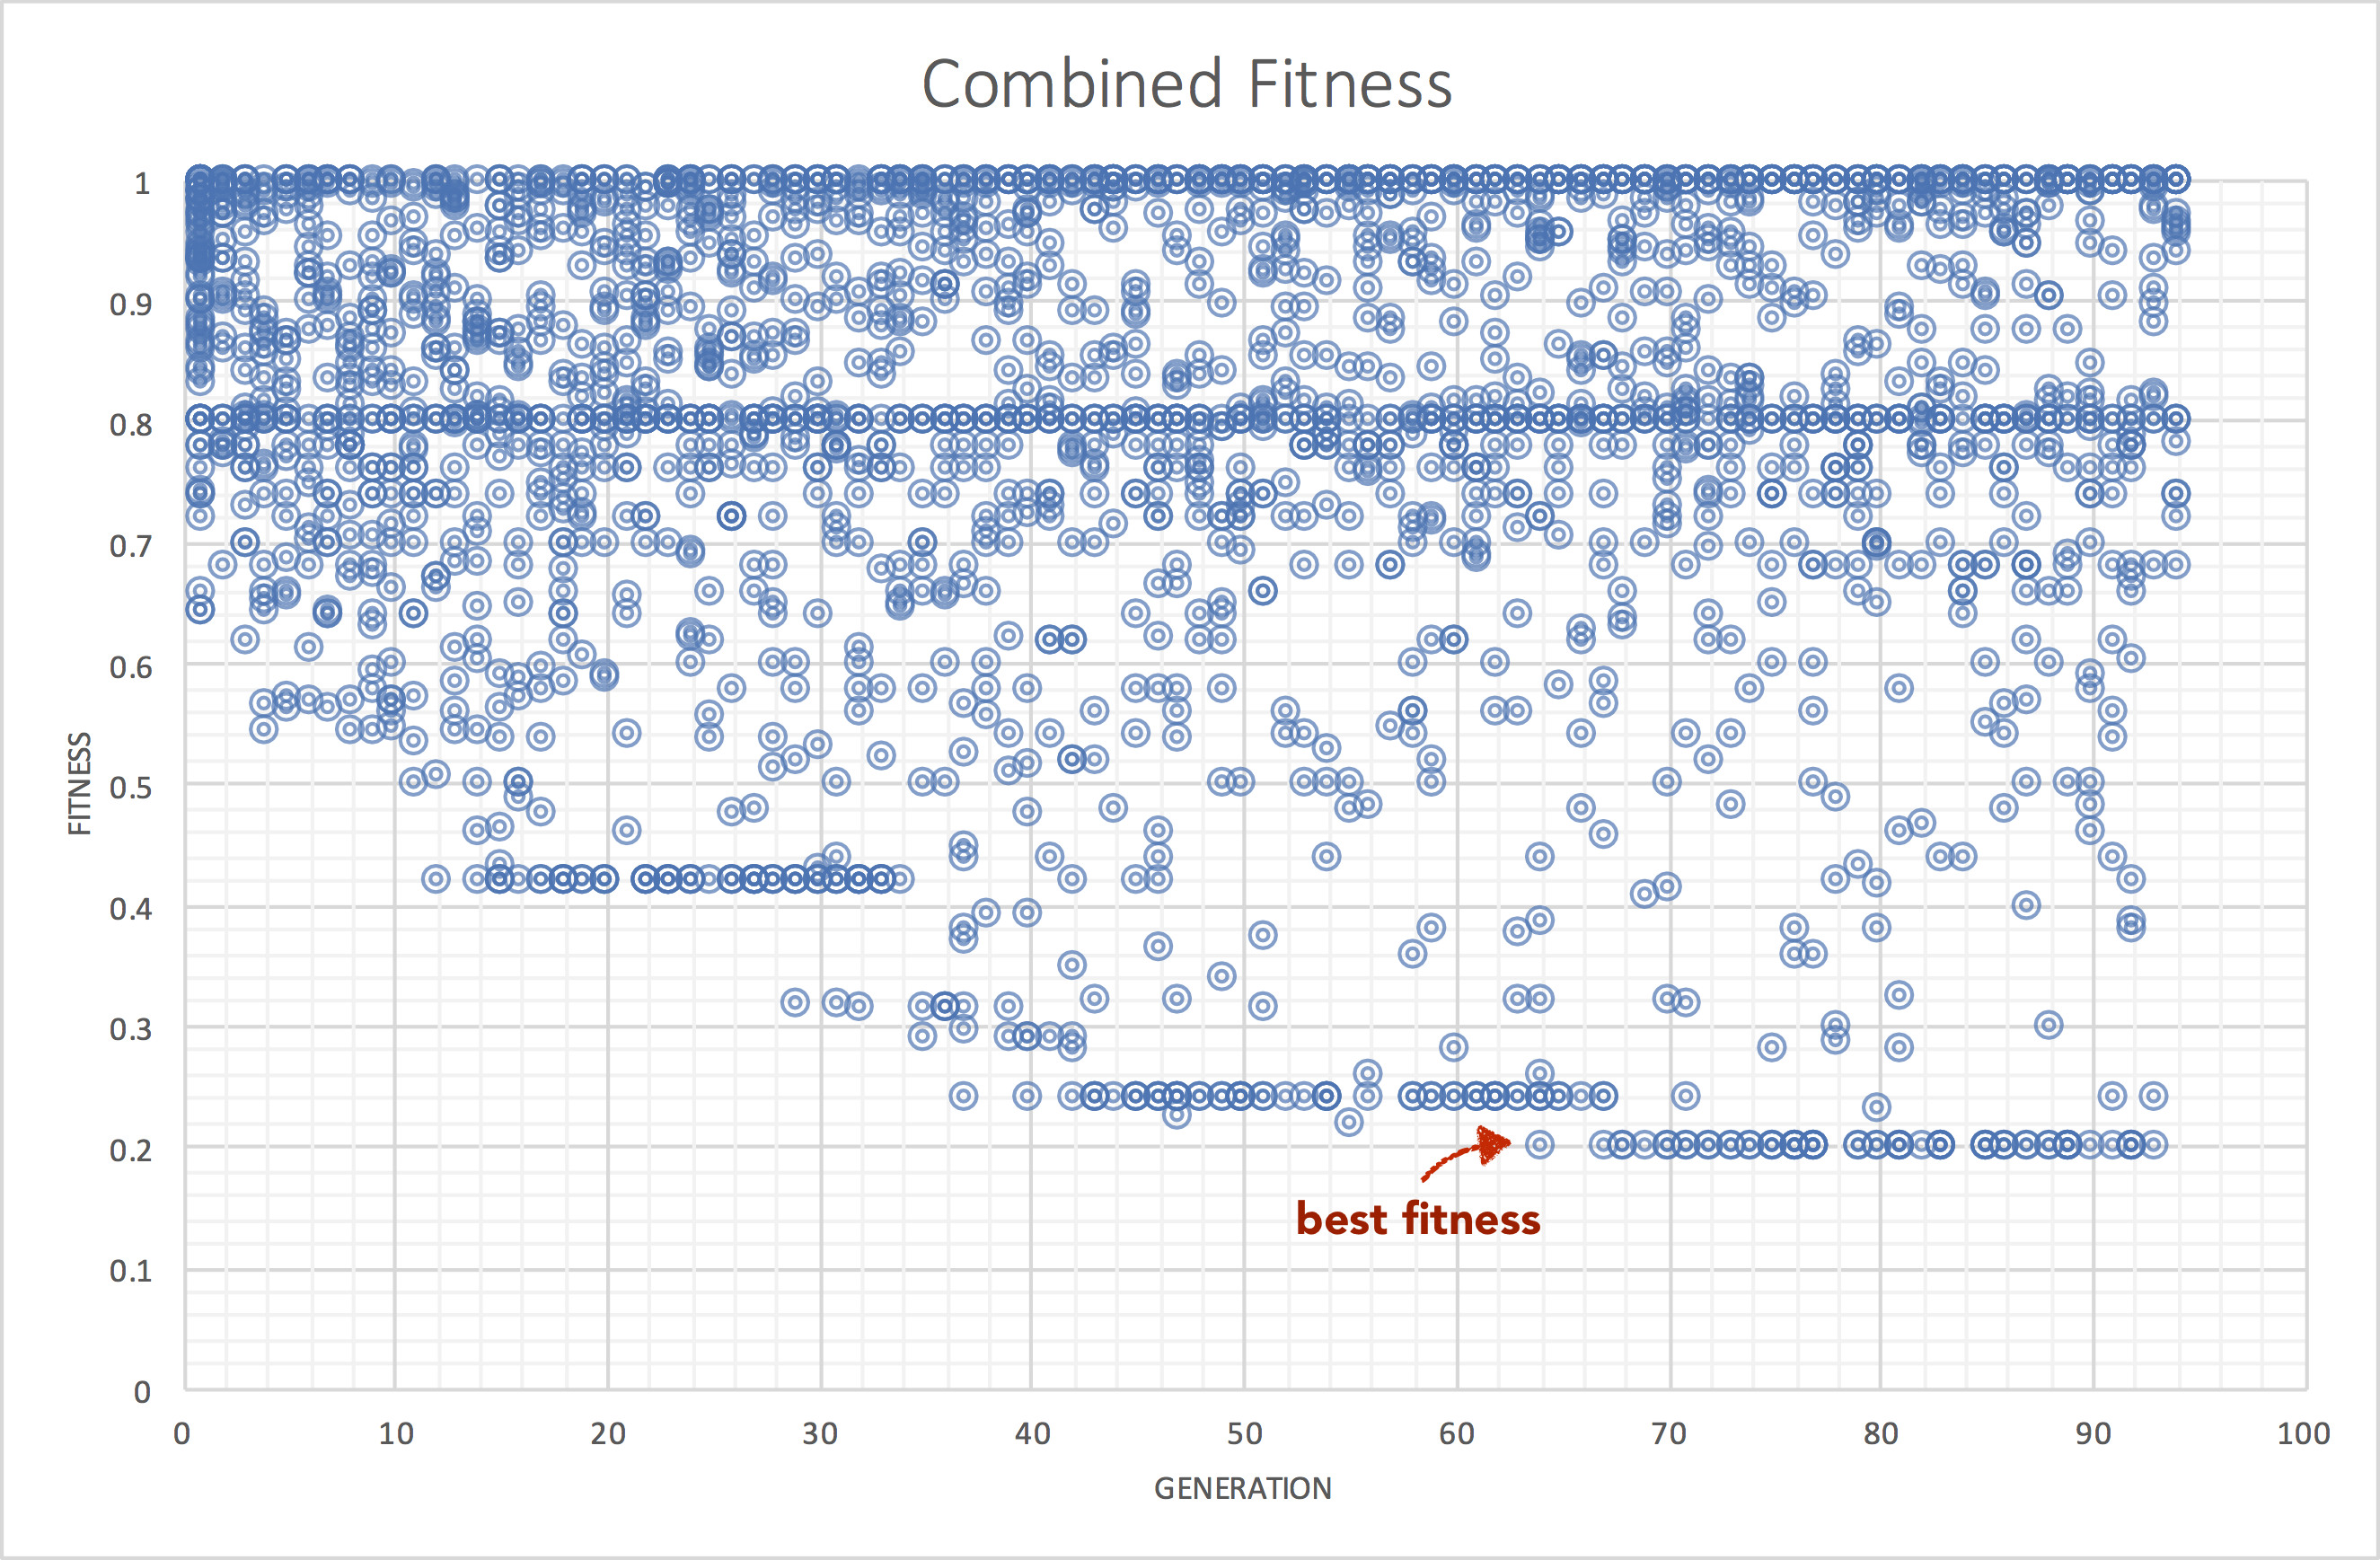
\includegraphics[width=0.8\linewidth]{figures/j-ga}
	\caption{The fitness of all generated battle systems, with respect to the combined objective, in the GA run that produced the system to be used in evaluation.}
	\label{fig:systemj}
\end{figure}

We then used the result of this run as a starting population for subsequent runs, in which the top-level fitness combinator was changed from \textit{min-max} to \textit{weighted average} and \textit{weighted-normalised geometric mean}. Comparing the results, it is not obvious which combinator produce the best result, as the best systems reported by these combinators all exist on the \textit{Pareto front} -- a set of points such that there exist no other point that is better than them in all dimensions\cite{marler2004survey} (see figure \ref{fig:combinators}). Any of these systems can be chosen as the generated balanced system, and we chose  the original system produced by the \textit{min-max} combinator.

\begin{figure}
	\centering
	\begin{subfigure}{0.6\textwidth}
		\centering
		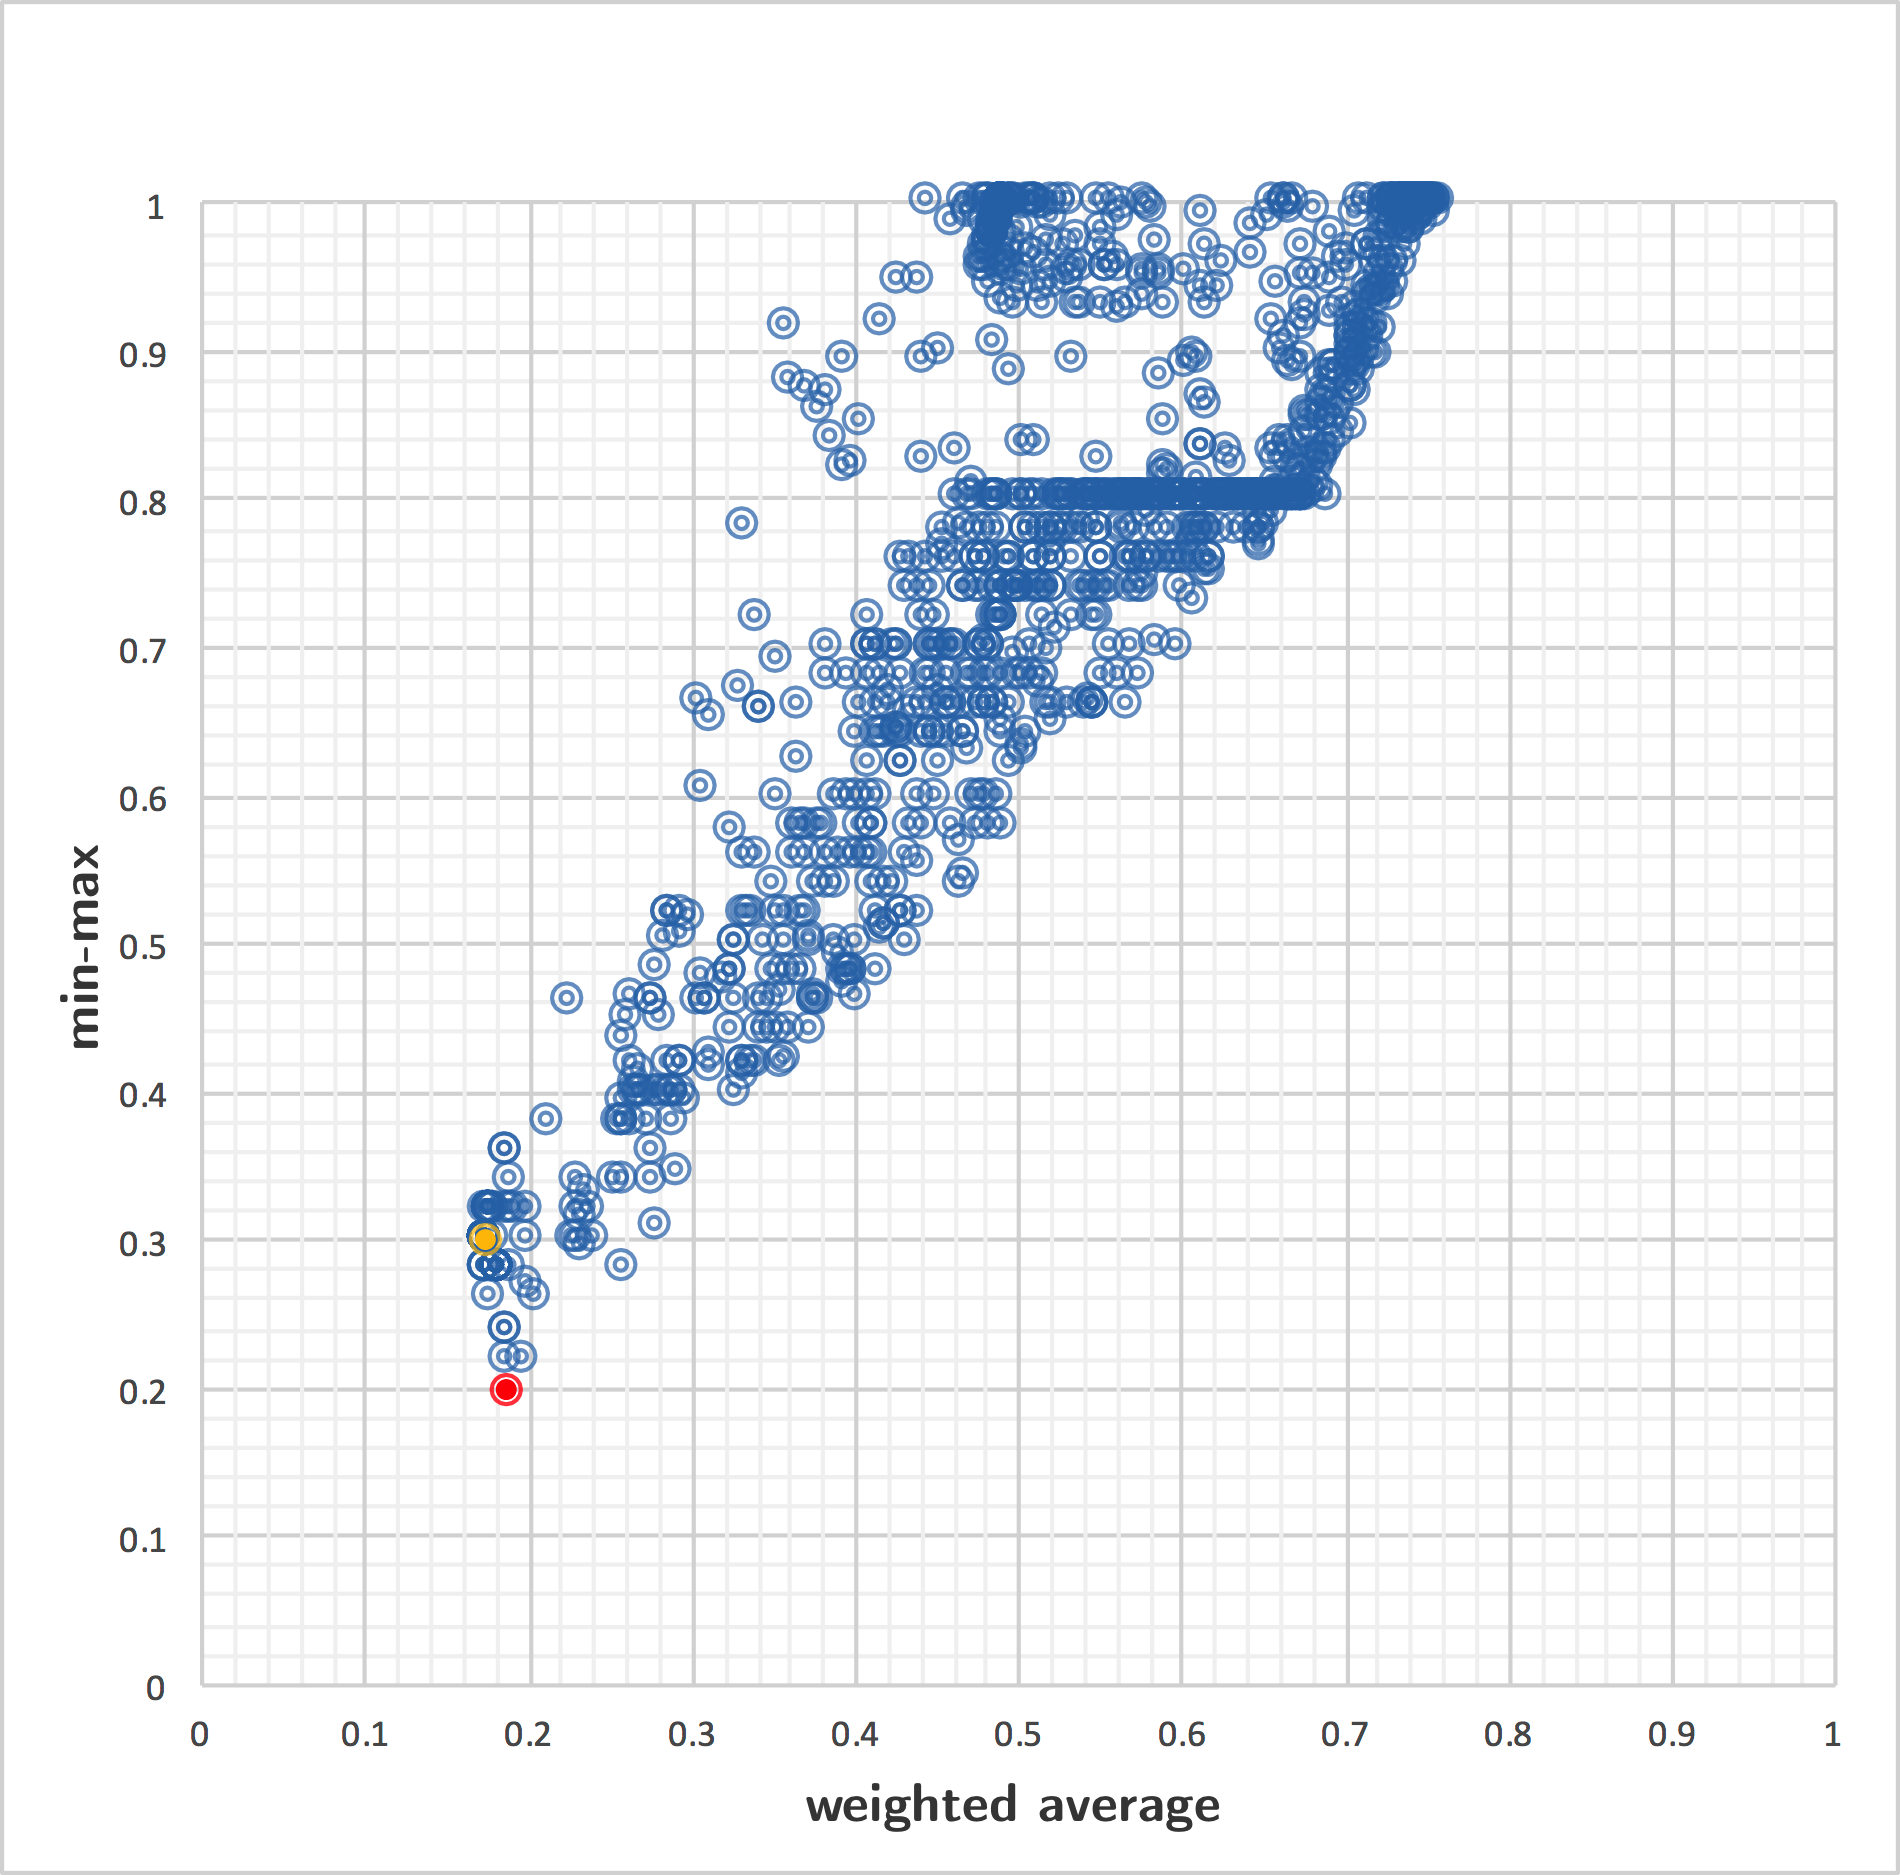
\includegraphics[width=1\linewidth]{figures/combinator_max_sum}
		\caption{Weighted average}
	\end{subfigure}
	\begin{subfigure}{0.6\textwidth}
		\centering
		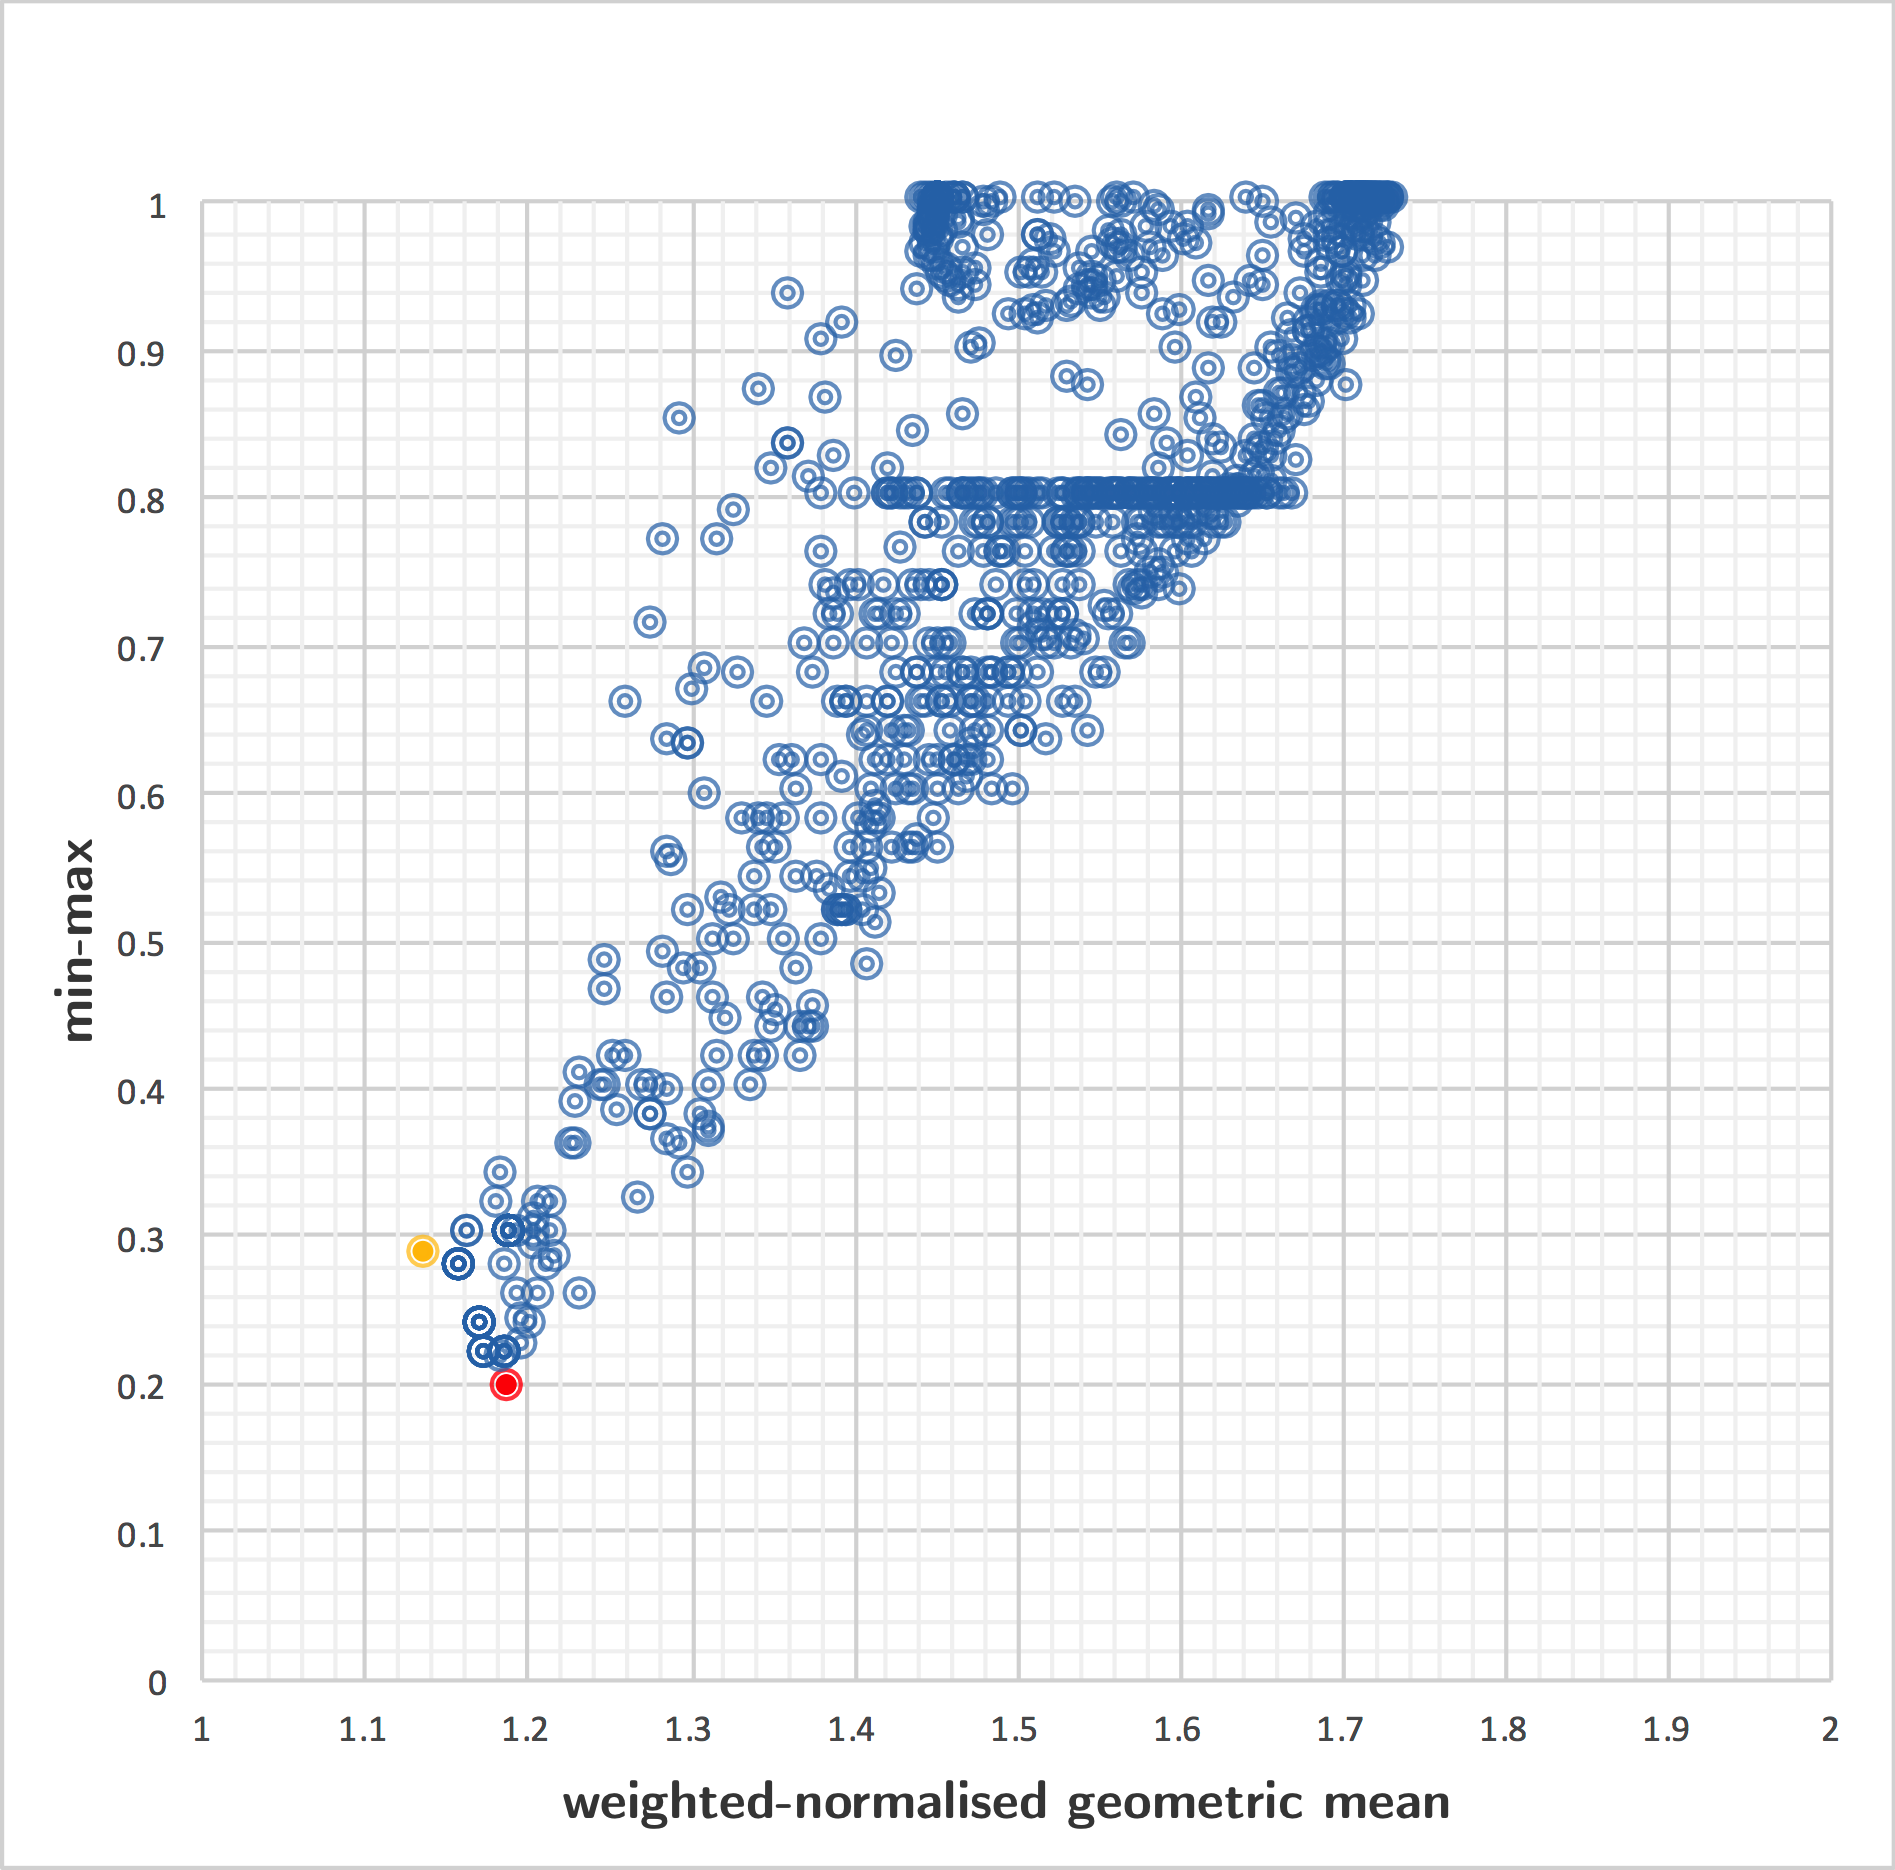
\includegraphics[width=1\linewidth]{figures/combinator_max_prod}
		\caption{Weighted-normalised geometric mean}
	\end{subfigure}
	\caption{Combinators comparison. The red points have the best fitness, according to \textit{min-max} combinator. The orange points are the best as reported by \textit{weighted average} and \textit{weighted-normalised geometric mean} combinators.}
	\label{fig:combinators}
\end{figure}

\subsubsection*{Unbalanced system}

The experiment needs another system to be compared with the generated one. We simply used the manually-created preliminary system that was recovered, as explained in section \ref{sub:recovery}.

We named the generated system as `system J', and the manually created system as `system H'. In table \ref{table:compare_hj} the objective fitnesses of the two systems are compared against each other, and also against another randomly generated system\footnote{The configuration for testing the two systems were: number of battles = 1000, battles are drawn at number of turns = 1000, random seed = 0. The random system was selected  from the starting populations of the two GA runs in the previous section, using the one whose min-max fitness is at the median.}. It can be seen that, in all the fitness combinators we have tried, the generated system is the most balanced, followed by the manually-created system, which is still more balanced that a random system.

\begin{table}
	\begin{tabu}{X[l5] X[c2] X[c2] X[c2]}
		\toprule
		objective & System J & System H & random\\ 
		\midrule
		\ warrior > ranger & 0.060 & 0.266 & 0.800\\
		\ ranger > mage & 0.018 & 0.200 & 0.720\\
		\ mage > warrior & 0.195 & 0.794 & 0.200\\
		\textbf{combat triangle} & 0.195 & 0.794 & 0.800\\
		\ anyone > cleric & 0.093 & 0.100 & 0.080\\
		\ team+cleric > team & 0.267 & 0.389 & 0.260\\
		\textbf{clerics as supporters} & 0.267 & 0.389 & 0.260\\
		\textbf{no first-mover advantage} & 0.008 & 0.015 & 0.060\\
		\textbf{appropriate damage} & 0.267 & 0.794 & 0.935\\
		\midrule
		combined (min-max) & 0.267 & 0.794 & 0.935\\
		combined (wgt. average) & 0.202 & 0.579 & 0.712\\
		combined (wgt. normalised geometric mean) & 1.199 & 1.557 & 1.683\\
		\bottomrule
	\end{tabu}
	\caption{Comparison of each sub-objective on systems J, H, and random.}
	\label{table:compare_hj}
\end{table}

\subsubsection*{User study}

The two systems were tested by human testers. We asked our 10 volunteers to download the solution and play around with the prototype, using both battle systems H and J. They were not told how these two systems are different. After that we asked them to fill out a questionnaire revolving around the feeling of balance. Full instruction and questionnaire can be found in appendix \ref{app:questionnaire}.

The respondents are:
\begin{itemize}
	\item mostly male (80\%)
	\item aged between 23-34 years old
	\item play games often (60\% play on a daily basis)
	\item quite familiar with the genre of tactical RPG (60\%)
\end{itemize}

\subsection{Results}

First we asked if the prototype can be classified as a TRPG game. Most (70\%) agreed, the rest said they were not sure.

We then proceeded to the main purpose of this user study -- to confirm that the battle system generated from the solution is more balanced than the one created manually. This was asked in a few different ways.

\subsubsection*{Direct question}

\begin{figure}
	\centering
	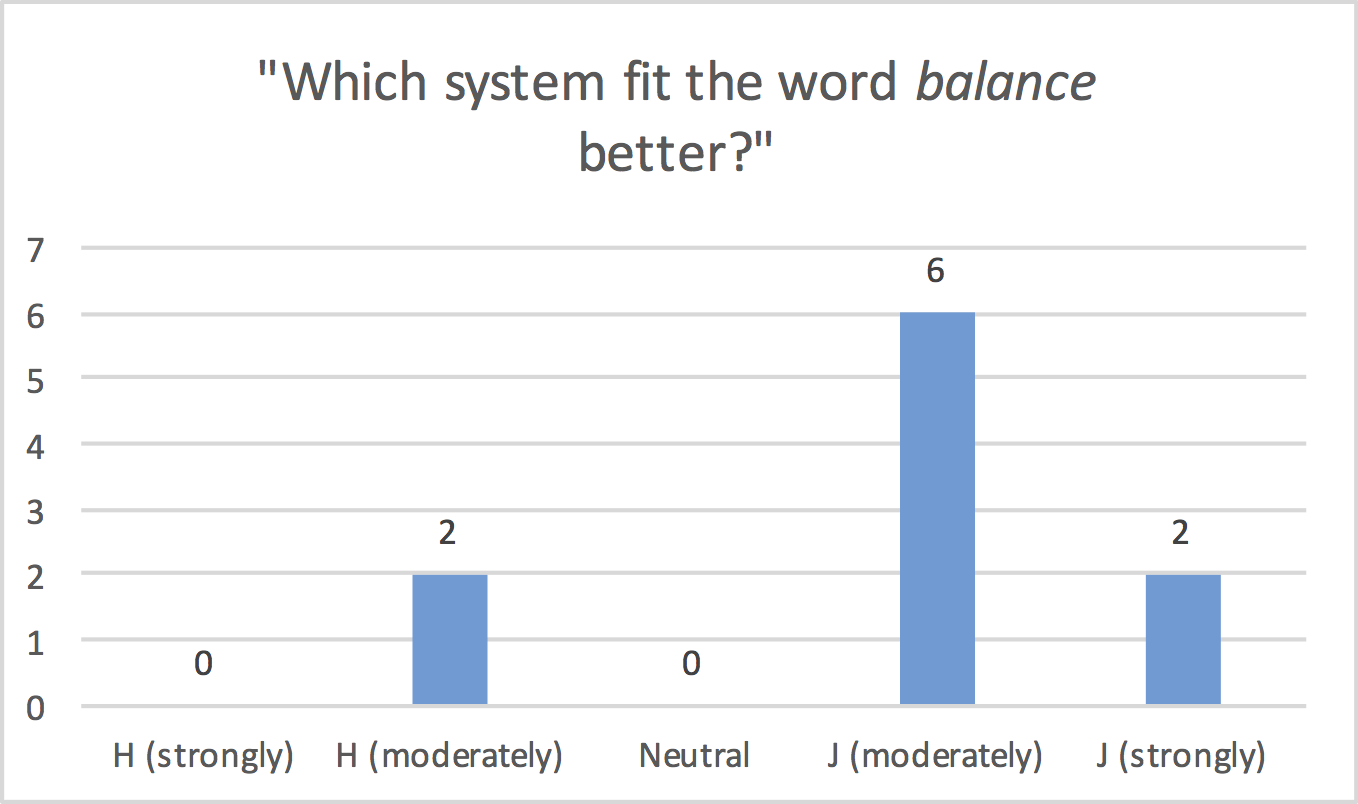
\includegraphics[width=0.6\linewidth]{figures/bar_balanced}
	\caption{Result of associating `balance' with the battle systems.}
	\label{fig:result_bar_balance}
\end{figure}

One of the question asks the respondents directly how they associate the term `balance' with the two battle systems. The result is as in figure \ref{fig:result_bar_balance}: 8 out of 10 respondents associated `balance' with the generated system, with 2 of them said the association is strong.

\subsubsection*{Balance as in `not overpowered'}

As noted in earlier chapters, there is no consensus on the precise definition of the word `balance'. Our interpretation is that a balanced system should not allow any unit to be too `overpowered' -- being able to beat all other units. The combat triangle was design according to this interpretation. The questionnaire did not define `balance', and thus it is possible that the volunteers might have a different interpretation than ours.

\begin{figure}
	\centering
	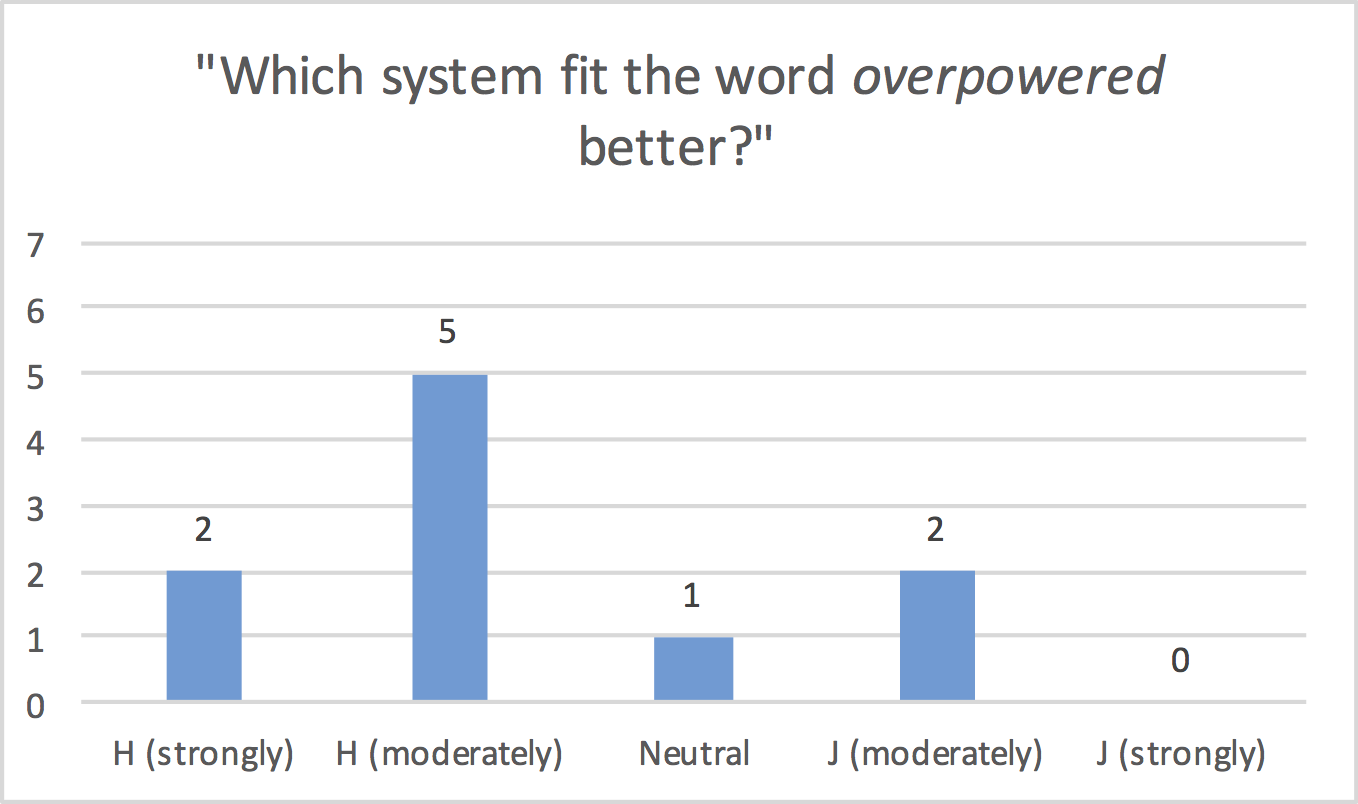
\includegraphics[width=0.6\linewidth]{figures/bar_op}
	\caption{Result of associating `overpowered' with the battle systems.}
	\label{fig:result_bar_op}
\end{figure}

For this reason, in addition to `balance', the respondents were also asked to associate `overpowered' with the two systems. The result is as in figure \ref{fig:result_bar_op}: 7 out of 10 respondents associated `overpowered' with the manual system, whereas 2 chose the generated system. This is a positive result -- the generated system is less overpowered.

As an anecdote, this does not necessarily mean that the respondents agree with our definition of balance. One of them said the generated system is \textit{both balanced and overpowered}, while another stated the opposite -- choosing the manual system for both characteristics. Investigating further, the responses were assign scores, as follows:
\begin{itemize}
	\item 1 for `System J (strongly)'
	\item 0.5 for `System J (moderately)'
	\item 0 for `Neutral'
	\item -0.5 for `System H (moderately)'
	\item -1 for `System H (strongly)'
\end{itemize}
It was then found that the correlation between \textit{balance} and \textit{overpowered} is merely -0.142, suggesting a weak negative relationship, while we expected a much stronger one.

\subsubsection*{Fun factor}

In addition to `balance' and `overpowered', respondents were also asked to associated `fun', `fast-paced', and `challenging' with the two systems. Using the same score assignment aforementioned, the correlation between `fun' and the others are:
\begin{itemize}
	\item Balance: 0.853
	\item Fast-paced: 0.829
	\item Overpowered: -0.010
	\item Challenging: -0.172
\end{itemize}

While this is not the result needed for differentiation of the two battle systems, it does justify our claim that \textit{balance is important for the enjoyment of the game}.

\subsubsection*{Party selection}

The questionnaire further asked the respondents to assemble a party of 4 units, choosing a combination of jobs that would be most likely to beat an AI party consists of one unit for each of the four jobs. We observed the following:

\begin{figure}
	\centering
	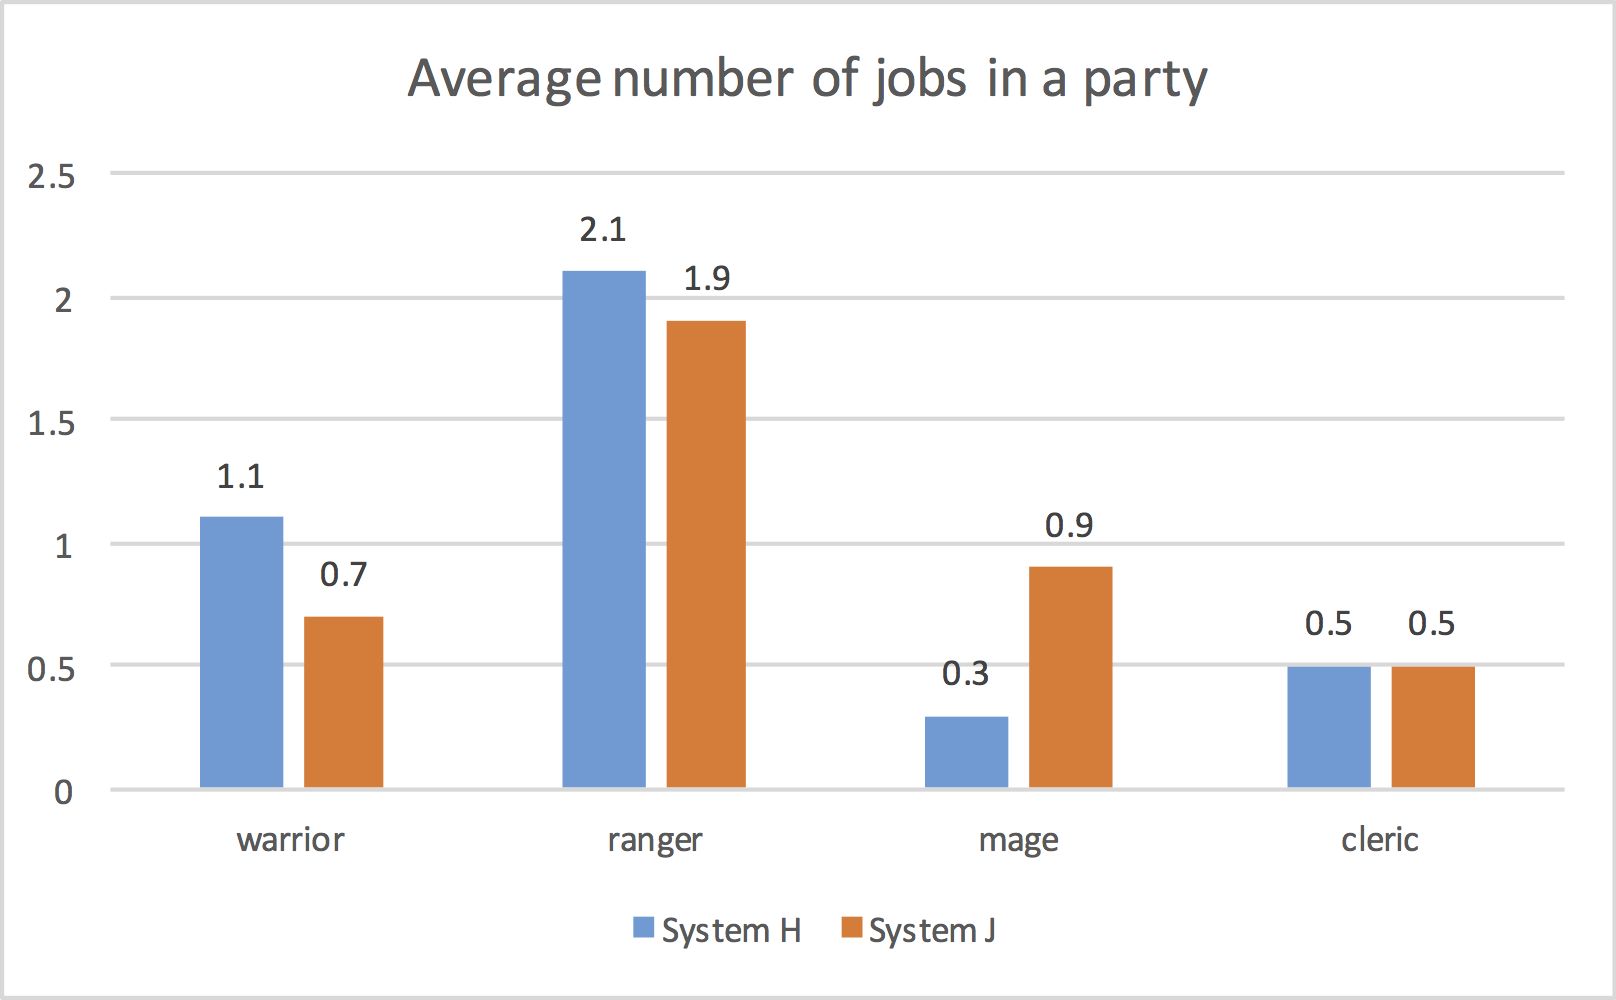
\includegraphics[width=0.6\linewidth]{figures/jobs_per_party}
	\caption{Distribution of jobs in the respondent-assembled parties.}
	\label{fig:jobs_per_party}
\end{figure}

\begin{itemize}
	\item For the three attacking character classes, the respondents perceived rangers to be the strongest by far, followed by warriors, then mages. This is true for both battle systems, but the disparity is more pronounced in the manually-created system than the generated one, as seen in figure \ref{fig:jobs_per_party}.
	
	\item We hypothesised that if a respondent can feel the presence of the combat triangle, then the assembled party should have at least one unit from each of the three attacking jobs. For system H (the manually-created one), only 1 out of 10 party qualifies for this criterion. System J does just a little better, with 2 qualified parties, but still far from what we expected from a balanced system. 
	
	Another hypothesis is that if the clerics-as-supporters objective is achieved, then the assembled party should consist of exactly one cleric. For both battle systems, half of the parties qualified for this criteria.
	
	Comparatively, the difference in the battle systems has no observable effect to the way the parties are assembled.
	
	\item An interesting fact is that, for 4 out of 10 respondents, their assembled parties for both battle systems are \textit{exactly the same}, despite them having clear distinction between the two systems, given their answers to other questions. This suggests that the perception of balance might not affect the party selection in the way we expected -- there could be other factors in the party formation decision (such as personal preferences to certain character classes).
\end{itemize}

In the end, we could not draw any conclusive result from this part of the questionnaire.

\section{Threats to validity}

This section identifies the threats to the validity of our results.

\begin{itemize}
	\item \textbf{Small size of respondents.} The number of respondents is 10. From statistical point of view, small sample size reduces the confidence level of the result.
	\item \textbf{Use of a single battle system to represent the solution.} The solution can produce a lot of battle systems. We generated a few and picked what we thought of as the best one for evaluation. This only proves (if the validation is justified) that the solution can generate a good battle system, but does not say anything about quality of battle systems produced by the solution in general.
\end{itemize}

\section{Summary}

In this section we evaluated the solution to the research question, by generating a battle system with the goal of balance, then asked a number of volunteers to compare it against an unbalanced system, without telling them which is which. Overall, most (70\%--80\%) of the 10 respondents agreed that \textbf{the generated system is more balanced and less overpowered}, even though the two terms are not as strongly correlated as we thought. However, balance does strongly imply enjoyment, justifying our position of using it as the optimisation goal. Contrary to our hypotheses, the perception of balance cannot be easily judged by how the players assemble their party. Finally we identified some threats that could undermine the validity of our result.
\chapter{Conclusion}

\section{Results and contribution}

This project started out asking if it is possible to create balanced battle systems for tactical RPG games in an automatic manner. To answer this question, we developed a solution with that capability, working on a prototypical game which was created to represent the battle part of a generic tactical RPG. The solution basically uses a generate-and-test approach, relying on genetic algorithm to generate good quality solutions. The approach requires an evaluation function (fitness function), in this case the function evaluates how balanced a battle system is. `Balance' in our interpretation is `not overpowered', so an ideal battle system should not allow a certain class of units to be too powerful, capable of beating everyone else. A population of random battle systems are then generated and evaluated. New systems are created from the old population, potentially with better fitness with each passing generation.

Computing the fitness of each battle system is a crucial part of this solution -- and in this case it is not trivial. Game content at this level of `game design', such as rules and mechanics -- including battle systems, are difficult to evaluate unless it is experienced in actual gameplays. The fitness function is therefore defined based on battle simulations, using a self-play AI. The quality of the fitness function depends directly on the quality of the AI, and we believe the AI we have built is quite competent.

The solution was then evaluated, by asking human volunteers to validate a generated balanced battle system, in comparison to a reference system that we manually created. Our solution assessed the two systems and reported that the one it generated is more balanced, and most of the volunteers agreed with that. With this confirmation, we can say that our solution is successful in creating a well-balanced battle system for a tactical RPG, fulfilling our purpose from the start.

\bigskip
Our contribution consists of the following artefacts, which completes all our primary objectives and most of the secondary ones:
\begin{itemize}
	\item A game prototype that incorporate most aspects of general TRPG battles, including races and jobs systems, complete with a graphical user interface.
	\item An AI that can play the game competently.
	\item The solution -- a procedural generation program capable of generating balanced battle systems.
\end{itemize}

The one secondary objective we did not fully complete is the one that asks for more complex battle mechanics. This is partially met, as while the following have not been included:
\begin{itemize}
	\item items, 
	\item equipment change,
	\item advanced magic spells, such as status abnormalities, and
	\item variation of terrain types,
\end{itemize}
We did, however, include the following extra elements to the game:
\begin{itemize}
	\item magic system as a rock-paper-scissors triangle of its own,
	\item terrain height affecting the attack actions, and
	\item complex turn order calculation.
\end{itemize}

In conclusion, we think this project is a success. We are able to create artefacts meeting most of the objectives, producing a battle system that is in balance, as validated from human perspectives.

\section{Future work}

In a sense, this project is a proof of concept that TRPG battle systems can be created using a procedural generation method. In this last section we suggest some directions that might improve this work further.

\subsection{Prototype generalisation}

The solution works on our battle prototype, which, though incorporating most aspects of TRPG battles, is still a single game. A simple extension would be to incorporate more elements into the prototype, or to parameterize more elements, turning them from being fixed parts of the game into parts of the battle system. Supporting more type of battle generator constraints is another possibility.

A more ambitious effort would see the prototype being generalised to describe a wide range of TRPG battles. One possible approach is to follow the direction existing researches in this area have been pursuing, by defining game description language that can describe a whole game genre, and use general game playing techniques to develop the AI part.

\subsection{Manifestation of the perception of balance}

All our conclusive results are based on subjective evaluation, from words association. The part that were meant to be a precise, objective quantification instead gave a rather inconclusive result. We framed the question based on the hypothesis that if the volunteers can sense the existence of balance, they would response by forming their parties in a certain way. In hindsight, this might not be true. It is possible that there is no significant correlation between balance and party formation. It is also possible that the correlation exists, but not in the way we assumed. Another possibility is that the way the question was asked might not properly address the correlation. Further exploration in this relationship would definitely have a consequence in the strength of our results.

%TC:ignore 

\begin{appendices}

\chapter{List of all derived attributes}
\label{app:attributes}

Derived character attributes are functions of one or two of the five basic attributes: STR -- strength, CON -- constitution, INT -- intelligence, WIS -- wisdom, DEX -- dexterity. 

\begin{tabu}{X[l2] X[l2] X[l4] }
	\toprule
	attribute & derived from & effects \\ 
	\midrule
	hit point (HP) & CON& Health point of the unit. Reduced upon being attacked.\\
	\addlinespace[0.2cm]
	magic point (MP) & WIS, INT& Spent to cast magic spells.\\
	\addlinespace[0.2cm]
	physical attack & STR, CON& Used to calculate damage when the unit is attacking physically.\\
	\addlinespace[0.2cm]
	physical defence & CON, STR& Used to calculate damage when the unit is being attacked physically.\\
	\addlinespace[0.2cm]
	magical attack & INT, STR& Used to calculate damage when the unit is doing magical attack.\\
	\addlinespace[0.2cm]
	magical defence & WIS, CON& Used to calculate damage when the unit is being attacked by magic.\\
	\addlinespace[0.2cm]
	evasion & INT, DEX& Used to calculate the chance of the attack being a hit or a miss.\\
	\addlinespace[0.2cm]
	speed & DEX& Used to calculate which unit get the next turn.\\
	move range & DEX, STR& Limit the number of cells the unit can move in a turn.\\
	\bottomrule
\end{tabu}

Derived weapon and armour attributes are functions of one or two of the material attributes: STR -- strength, CRF -- craftsmanship, PLS -- plasticity, ENC -- enchantment.

\bigskip
Weapon attributes:

\begin{tabu}{X[l2] X[l2] X[l4] }
	\toprule
	attribute & derived from & effects \\ 
	\midrule
	physical enhancement & STR, CRF & Enhancing physical attack.\\
	\addlinespace[0.2cm]
	magical enhancement & ENC & Enhancing magical attack.\\
	\bottomrule
\end{tabu}

\bigskip
Armour attributes:

\begin{tabu}{X[l2] X[l2] X[l4] }
	\toprule
	attribute & derived from & effects \\ 
	\midrule
	physical enhancement & PLS, CRF & Enhancing physical defence.\\
	\addlinespace[0.2cm]
	magical enhancement & ENC & Enhancing magical defence.\\
	\bottomrule
\end{tabu}

\chapter{Building and running the solution}

\section{Build from source files}

System requirements for the build machine:
\begin{itemize}
	\item Apache Maven. We tested with version 3.2.5.
	\item Java Development Kit 8.
\end{itemize}

To build the solution, simply navigate from the command line to the project root folder, the one containing \texttt{pom.xml} file. Then enter this command:
\begin{tcolorbox}
	\texttt{mvn package}
\end{tcolorbox}
This would compile the source files, run a \textit{TestNG} test suite, and package into 2 .jar files, one with dependencies included and one without.

\section{Run}

System requirements for the executing machine:
\begin{itemize}
	\item Java Runtime Environment 8.
\end{itemize}

The build process would package the whole solution into a .jar file, named \texttt{SRPG-<version>-jar-with-dependencies.jar}. For conciseness we will refer to this file as \texttt{SRPG.jar}.

The program can be run in 4 different modes.

\paragraph{Volunteer mode.} This is the mode intended to be used by the volunteers to evaluate the battle systems. By double-clicking on the .jar file (on systems that support launching by double-clicking), or running from the command line:
\begin{tcolorbox}
	\texttt{java -jar SRPG.jar}
\end{tcolorbox}
This would launch the evaluation process, as described in section \ref{sub:guiextension}.

\paragraph{Observation mode.} This is the original mode from phase \rom{1} of the implementation. It is retained for the use of testing and observing AI behaviours. To use this mode, enter the following to the command line:
\begin{tcolorbox}
	\texttt{java -jar SRPG.jar observe [options]}
\end{tcolorbox}
where the options are:
\begin{itemize}
	\item \texttt{-system [path to battle system]} -- the battle system to observe
\end{itemize}
This would launch a screen where the two players can be selected. Click `start', and the battle screen will be displayed.

\paragraph{Battle system evaluation mode.} This is used to evaluate a battle system against an objective, as we have done in section \ref{sub:meth}. To use this mode, enter the following to the command line:
\begin{tcolorbox}
	\texttt{java -jar SRPG.jar eval [options]}
\end{tcolorbox}
where the options are:
\begin{itemize}
	\item \texttt{-system [path to battle system]} -- the battle system to evaluate
	\item \texttt{-count [number]} -- the number of battles to be simulated (default: 10)
	\item \texttt{-turnsLimit [number]} -- the maximum turns allowed for a battle before it would be judged as a draw. If not present, the battles would be allowed to go on as long as it needs, potentially forever.
	\item \texttt{-objective [path to the objective file]} -- the objective tree
	\item \texttt{-seed [number]} -- the random seed to be used in this process (default: 0)
\end{itemize}

Running the program in this mode would print a detailed evaluation for all sub-objectives in the objective tree to the standard output.

\paragraph{Genetic algorithm mode.} This mode runs the genetic algorithm process to create a balanced battle system. To use this mode, enter the following to the command line:
\begin{tcolorbox}
	\texttt{java -jar SRPG.jar ga [options]}
\end{tcolorbox}
where the options are:
\begin{itemize}
	\item \texttt{-count [number]} -- the number of battles to be simulated for each matchup (default: 10)
	\item \texttt{-turnsLimit [number]} -- the maximum turns allowed for a battle before it would be judged as a draw. Like in the evaluation mode, it is possible to omit this option, but this is strongly not recommended, as it could easily stall the whole GA process.
	\item \texttt{-objective [path to the objective file]} -- the objective tree (default: models/objective.json)
	\item \texttt{-seed [number]} -- the random seed to be used in this process (default: 10)
	\item \texttt{-size [number]} -- the population size (default: 30). If this is omitted, \texttt{-population} must be present.
	\item \texttt{-population [path to population file]} -- the starting population. If this is omitted, \texttt{-size} must be present.
	\item \texttt{-maxGen [number]} -- the maximum number of generation (default: 100)
	\item \texttt{-steadyGen [number]} -- the process would stop if this number of generation has passed without producing better fitness (default: 20)
\end{itemize}

The program would print the number of generations that have been processed to the standard output. Detailed data will also be printed to files, with \texttt{log.csv} containing summary result of each generation, and \texttt{data.csv} containing fitness values for each individual battle system. If the process stops successfully, it would produce two more files: \texttt{bestsys.json} for the resulting battle system, and \texttt{population.xml}, for the whole population of the last generation, which can be used as starting population for subsequent runs.

\chapter{Game references}

\printglossaries

\chapter{Questionnaire}
\label{app:questionnaire}

\textbf{Google Forms} was used in our users study. All responses were collected from the online form. The print version of the instruction and the questionnaire are presented here.

\includepdf[pages=-,pagecommand=\thispagestyle{plain},scale=0.7,frame=true]{resources/instruction.pdf}

\includepdf[pages=-,pagecommand=\thispagestyle{plain},scale=0.7,frame=true]{resources/evaluation_form.pdf}


\end{appendices}
\printbibliography

%TC:endignore 

\end{document}   